\documentclass[a4paper,12pt]{report}

% Page Layout
\usepackage{geometry}
\geometry{
  a4paper,
  left=20mm,
  right=20mm,
  bottom=15mm,
  top=20mm
}
\usepackage{Archivo}
\usepackage[T1]{fontenc}
\sffamily

\usepackage{graphicx, wrapfig, xcolor, multicol}
\usepackage{tikz, pgfplots}
\usepgflibrary{shadings}
\usetikzlibrary{positioning, shapes.geometric, fit}
\pgfplotsset{compat=1.18}
\usepackage{amsmath, amssymb, amsthm, mathtools}
\usepackage[most]{tcolorbox}
\graphicspath{{images/}}

\linespread{1.3}
\usepackage{url}
\urlstyle{same}
\usepackage{hyperref}
\hypersetup{
    colorlinks=true,
    linkcolor=blue,
    filecolor=magenta,
    urlcolor=cyan,
  }


% ------------------------------------------------------------------------------------------------------------------
\begin{document}
\begin{center}
 \bfseries \Large A two-days workshop on \\
  Climate Change:  Modelling,  Mitigation,  and  Adaptation
\end{center}
\vspace{5mm}
The Central Department of Mathematics, Institute of Science and Technology , Tribhuvan University, Kathmandu Nepal organized a two-days workshop on Climate Change:  Modelling,  Mitigation, and  Adaptation. The workshop started off on fourth April, 2024 Thursday and completed successfully on fifth  April, 2024 Friday which took place inside the Central Department of Mathematics, TU, Kritipur, Nepal.
\vspace{5mm}

\begin{figure}[h!]
  \centering
  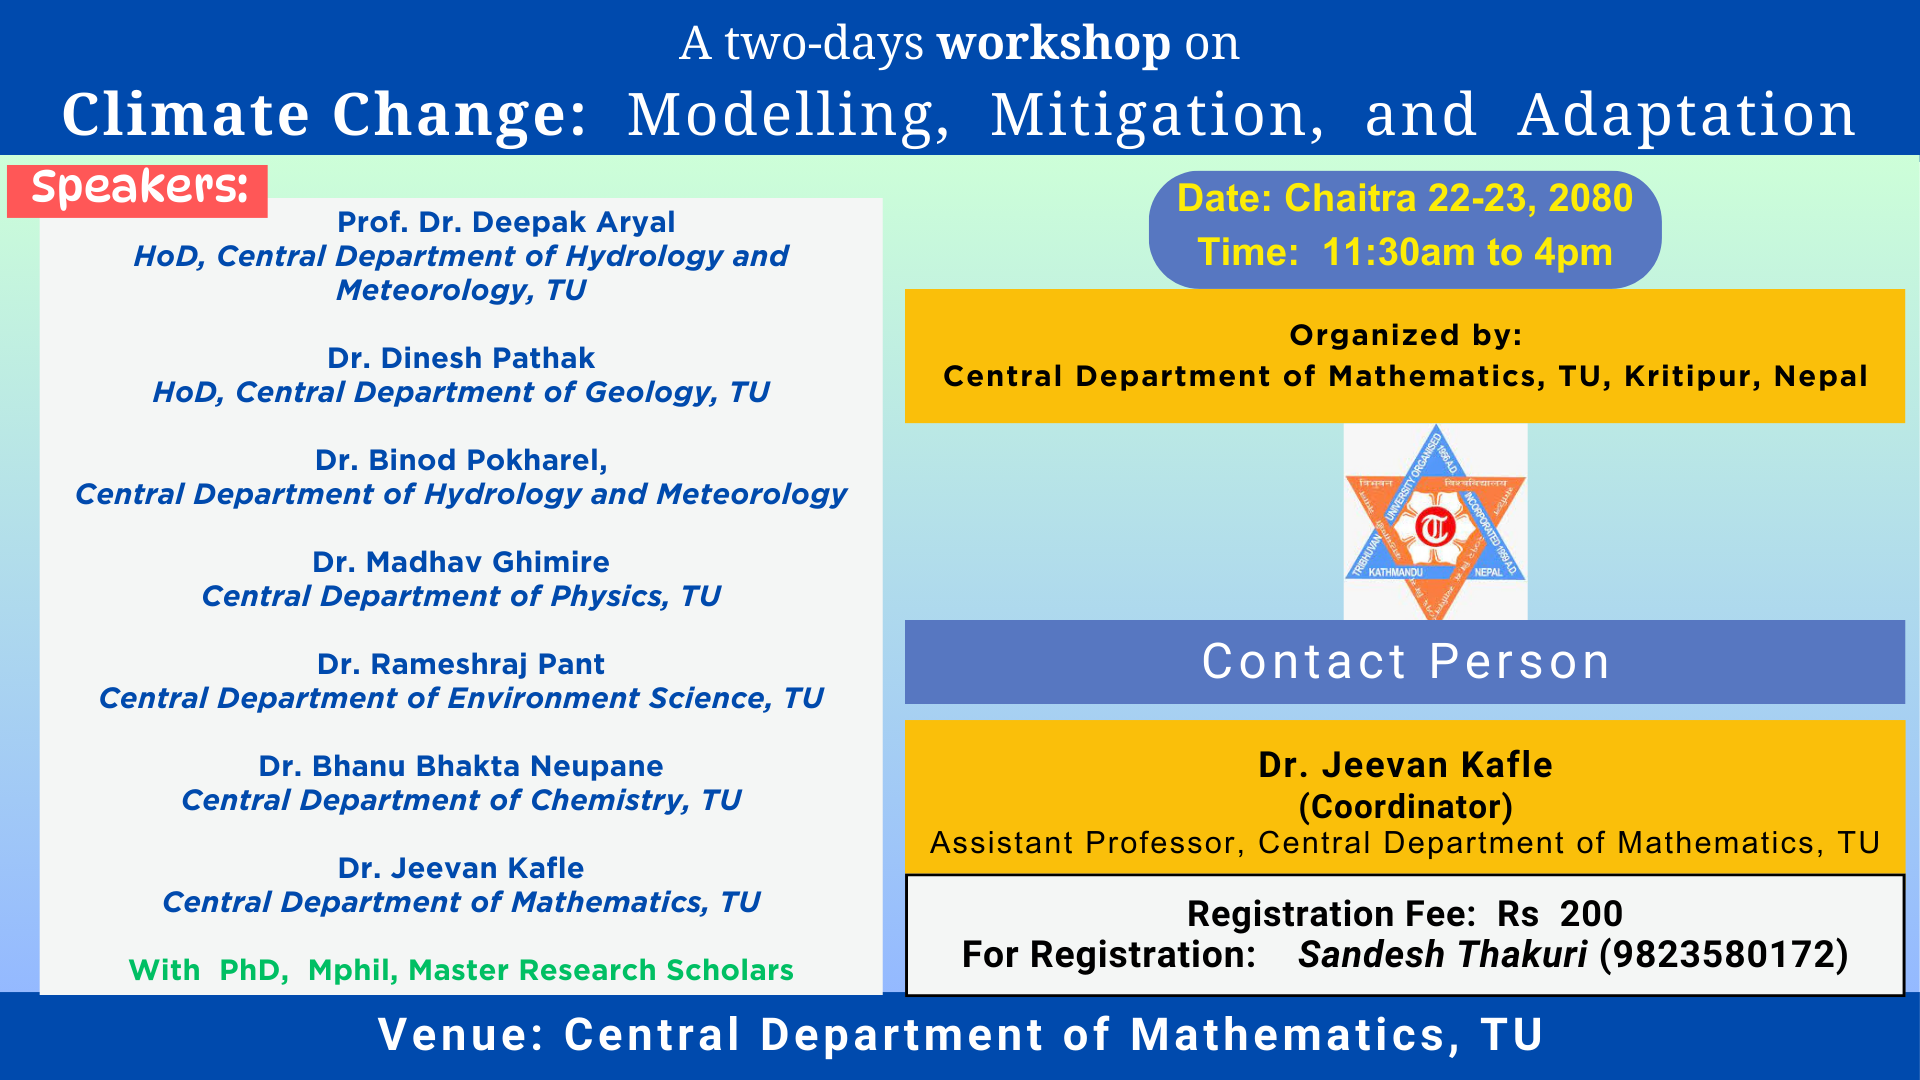
\includegraphics[scale=0.33]{workshop_climatechange.png}
\end{figure}
\vspace{5mm}
\noindent
The chairman of the workshop was the HoD Prof. Dr. \textbf{Chet Raj Bhatta}. The workshop was coordinated by \textbf{Dr. Jeevan Kafle} who is a leading figure in mathematics and a faculty of the Central Department of Mathematics, TU whose area of research is modelling in natural and applied sciences. The organizing team  consisted of \textbf{CDM Student Council} who took all the management responsibilities of the workshop under the leadership of the President of the Council \textbf{Mr. Sandesh Thakuri}. Other members of the team were:
\vspace{10mm}

\begin{minipage}{0.45\textwidth}
 \begin{itemize}
\item Sec. Manoj KC
\item Mem. Ranjan Kumar Chaudhary
\item Surendra Chaudhary
\end{itemize}
\end{minipage}\hspace{3mm}
\begin{minipage}{0.45\textwidth}
\begin{itemize}
\item VP. Biddha Pokhrel
\item Treasurer. Dhakaram Regmi
\item Mem. Jayanti Saud
\end{itemize}
\end{minipage}

\vspace{5mm}
\noindent
The Chief-Guest of the workshop was the Dean of IoST, TU Prof. Dr. \textbf{Binil Aryal}.
\clearpage
\noindent
Note books for the workshop was sponsored by the \textbf{Everest Engineering College, Kathmandu, Nepal}.\\
The workshop consisted of both online and physical sessions and a CDM alumni talk series session at the end. Seven experts from various central departments of TU came together to train during the workshop. The list of experts was as follows:


\begin{table}[h!]
\centering
  \begin{tcolorbox}[colframe=blue!52, colback=white, width=\linewidth]
\centering  \footnotesize
\begin{tabular}{l||c}

    1. Prof. Dr. Deepak Aryal &
    \textit{HoD, Central Department of Hydrology and Meteorology, TU}\\
    \\
    2. Dr. Dinesh Pathak &
    \textit{HoD, Central Department of Geology, TU}\\
    \\
    3. Dr. Binod Pokharel &
    \textit{Central Department of Hydrology and Meteorology}\\
    \\
    4. Dr. Madhav Ghimire &
    \textit{Central Department of Physics, TU}\\
    \\
    5. Dr. Rameshraj Pant &
    \textit{Central Department of Environment Science, TU}\\
    \\
    6. Dr. Bhanu Bhakta Neupane &
    \textit{Central Department of Chemistry, TU}\\
    \\
    7. Dr. Jeevan Kafle &
    \textit{Central Department of Mathematics, TU}\\
    \end{tabular}
  \end{tcolorbox}
\end{table}
\noindent
There was a guest appearance of a Professor from the South Asian University on the first day and a CDM alumni talk from Prof. Dr. Kedar Nath Upreti on the second day. Other guests were the President of Nepal Mathematical Society Prof. Dr. Narayan Prasad Pahari and various personal from Kathmandu University on the first day and various alumnus of this department on the second day. This workshop was attended by around \textbf{100 participants} from various central departments of TU and various campuses of TU and from Kathmandu University.

\vspace{5mm}
\begin{figure}[hb!]
  \centering
  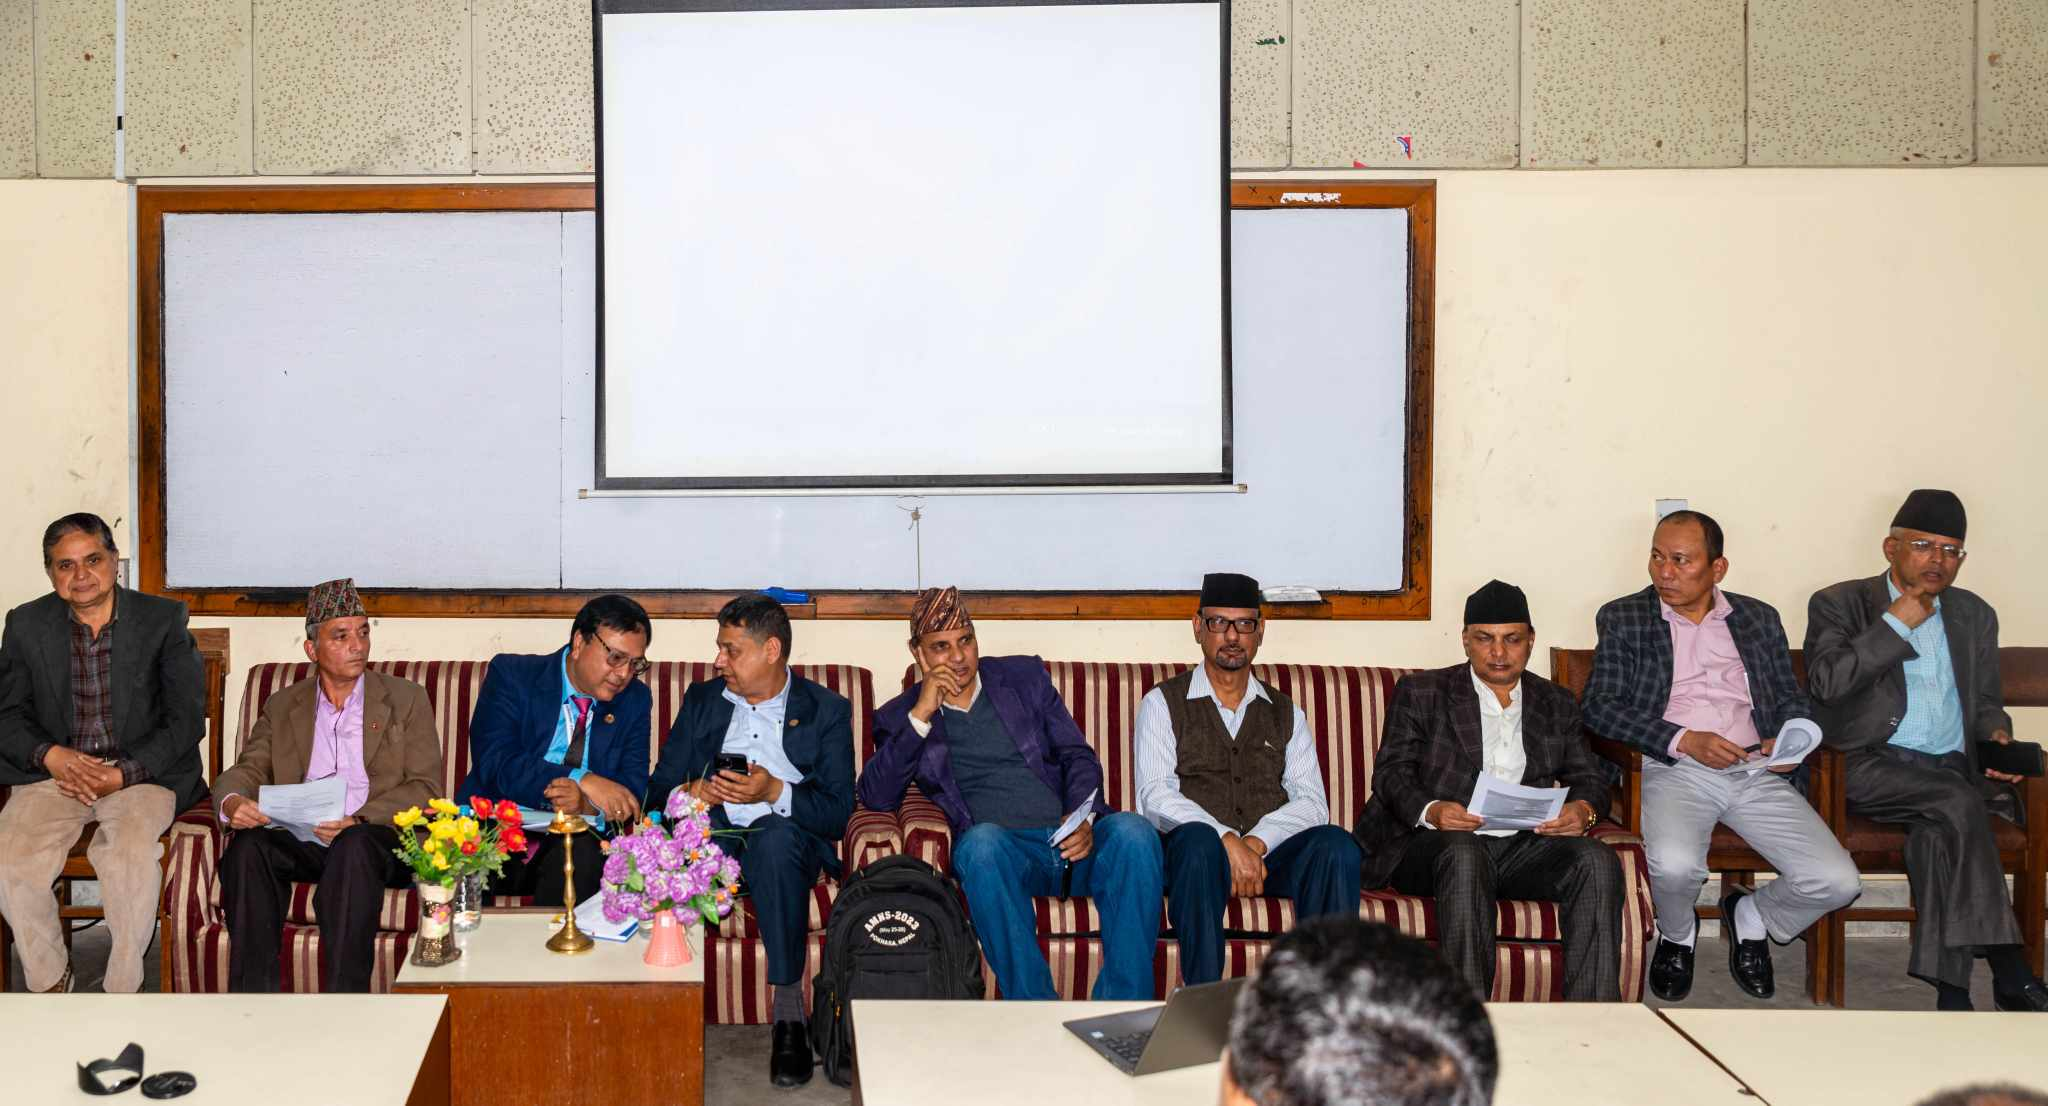
\includegraphics[width=15cm, height=8cm]{guest.jpg}
\end{figure}
\clearpage

{\Large \textbf{Objectives}}\\

This workshop was organized with the following objectives:
\begin{itemize}
\item Discuss Climate Change from various aspects
\item Foster Collaborative Research
\item Enhance Interdisciplinary Research
\item Interaction between various departments of TU
\item Interaction between Masters, MPhil and PhD Students.
\end{itemize}

\vspace{15mm}

\begin{figure}[h!]
  \centering
  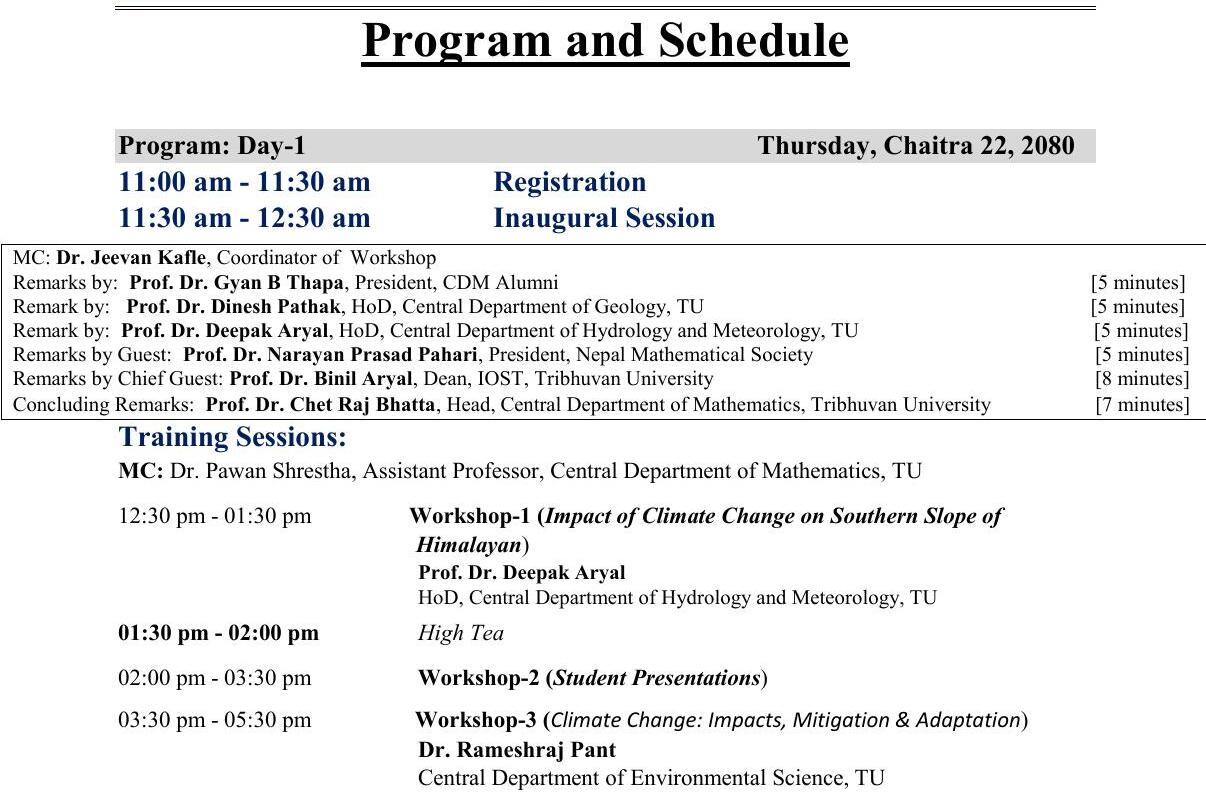
\includegraphics[width=17.5cm, height=15.5cm]{p1.jpg}
\end{figure}
\clearpage


\begin{figure}[h!]
  \centering
  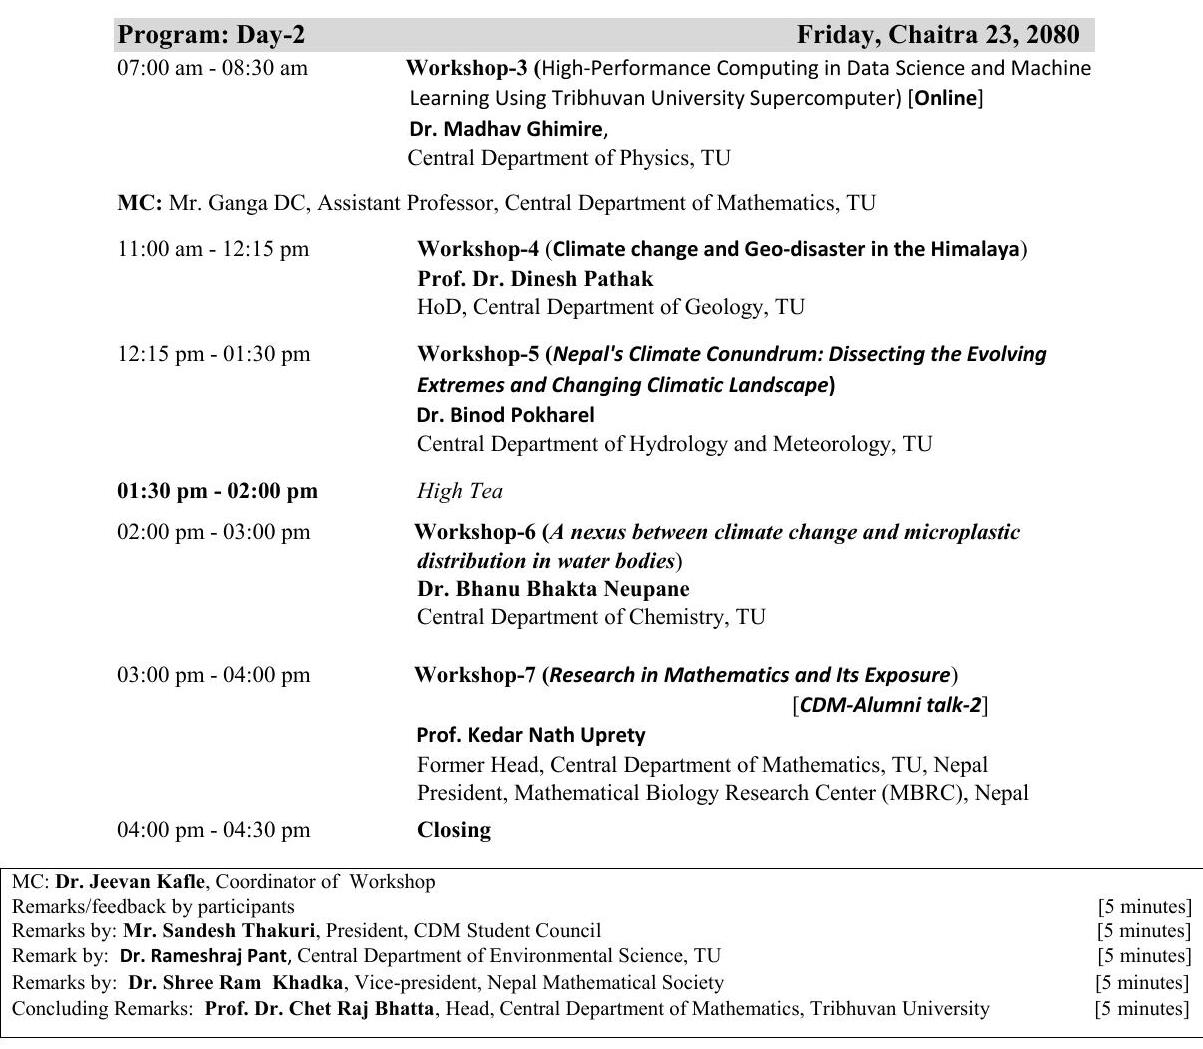
\includegraphics[width=17.5cm, height=18.5cm]{p2.jpg}
\end{figure}

\begin{minipage}{0.45\textwidth}
  The workshop had to be conducted by the Mathematics Department because at the heart of every research and problem solving tool there is mathematics. The workshop is about modelling, mitigation and adaptation. Every kind of scientific modelling is mathematics.
\end{minipage} \hspace{5mm}
\begin{minipage}{0.41\textwidth}
  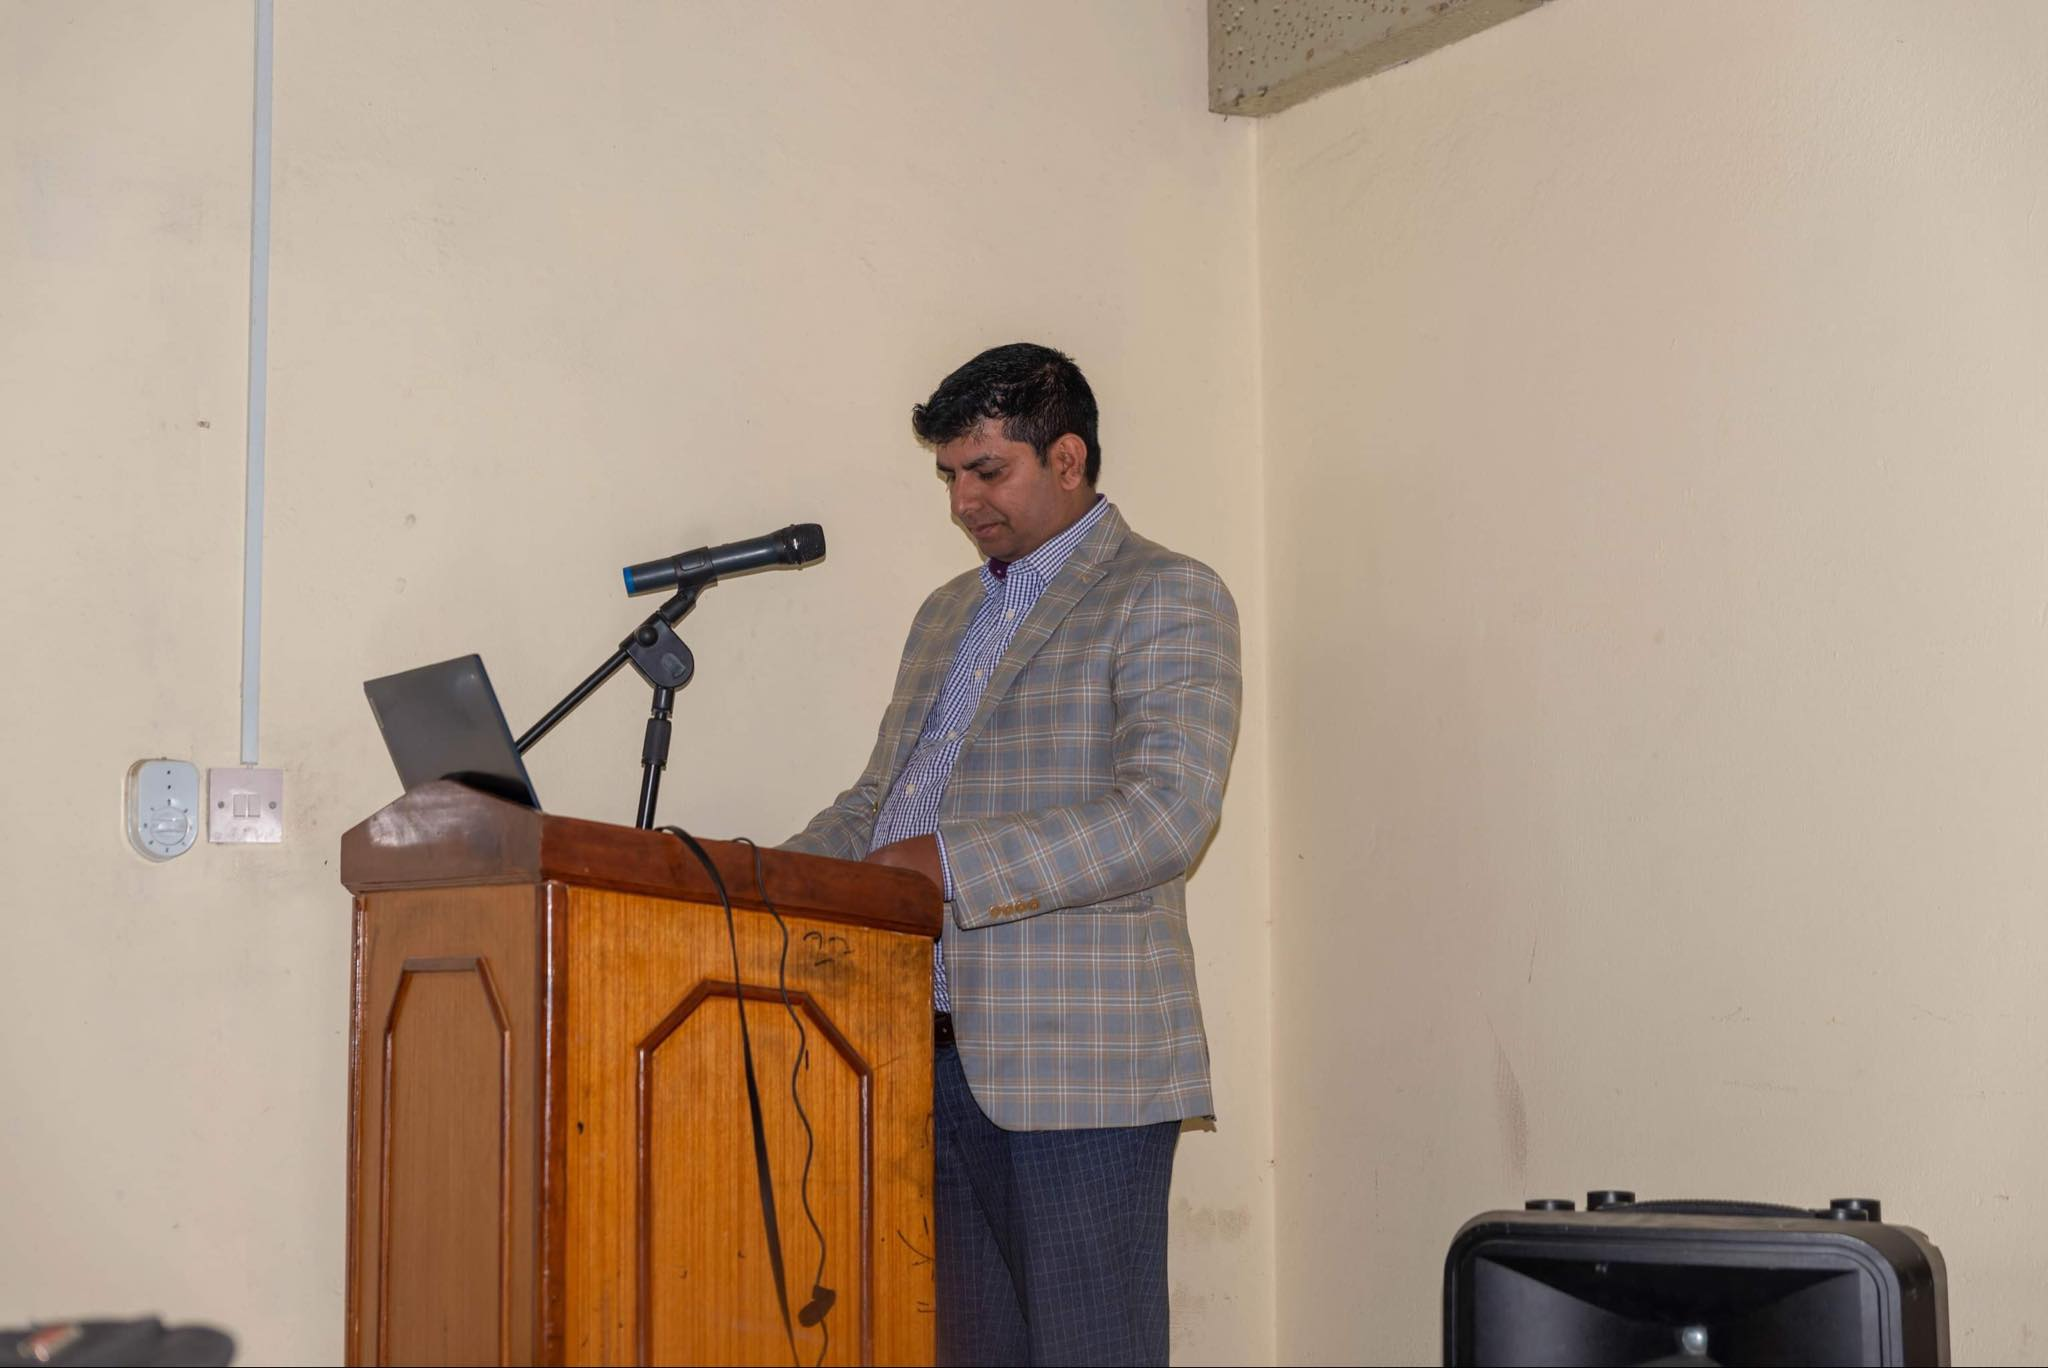
\includegraphics[width=7.3cm, height=5.5cm]{jeevan.jpeg}
 \hspace*{5mm} Dr. Jeevan Kafle
 \end{minipage}



\clearpage

{\bfseries \Large Inaugural Session}\\[3mm]
The workshop was inaugurated by the Chief-Guest and the Chairman of the workshop along with the distinguished guests at 11:45am. The Chief-Guest stressed on the increasing importance of mathematics in applied sciences. He mentioned that the real-world is chaotic, so the recent trend is to use statistical ways and the very recent trend is to use data-science because statistical ways is insufficient to handle huge data in applied sciences.

\vspace*{4mm}

\begin{figure}[h!]
  \centering
  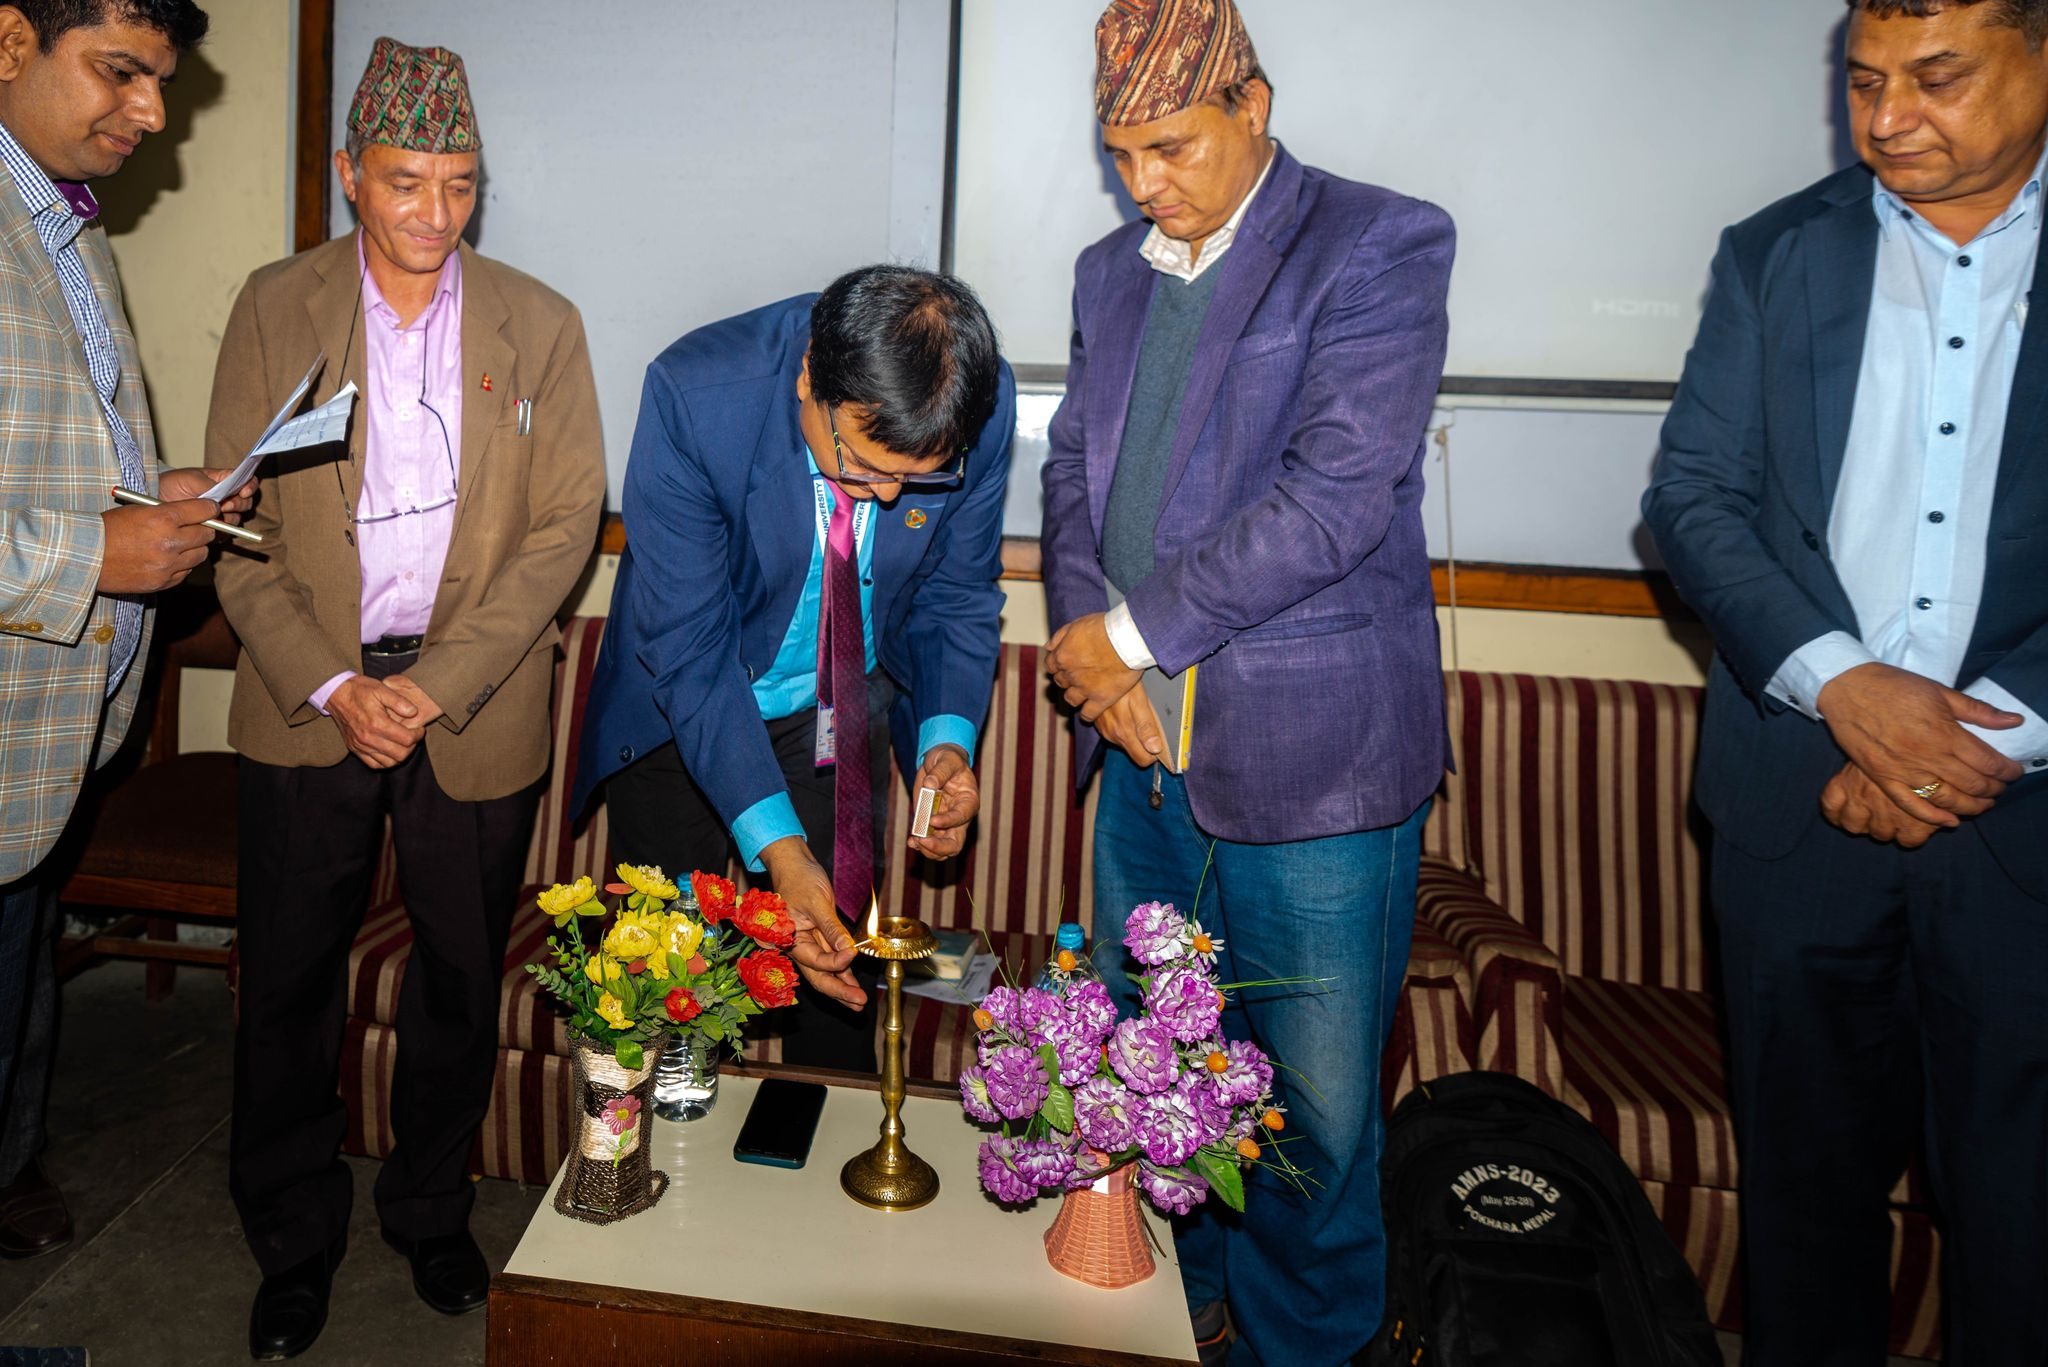
\includegraphics[width=15cm, height=5.9cm]{inauguration.jpg}
\end{figure}

\vspace*{5mm}

\noindent
The Head of the Department of Hydrology and Meteorology, TU Prof. Dr. Deepak Aryal was one of the special guest; this workshop being a workshop on climate change. He spoke to the young researchers to focus on the modelling aspects of research and mathematics is the heart of modelling. He encouraged the young mathematicians to not just sit in the classroom and solve the book problems but to go to real world where mathematicians are more needed.

\vspace{3mm}
\begin{multicols}{2}
  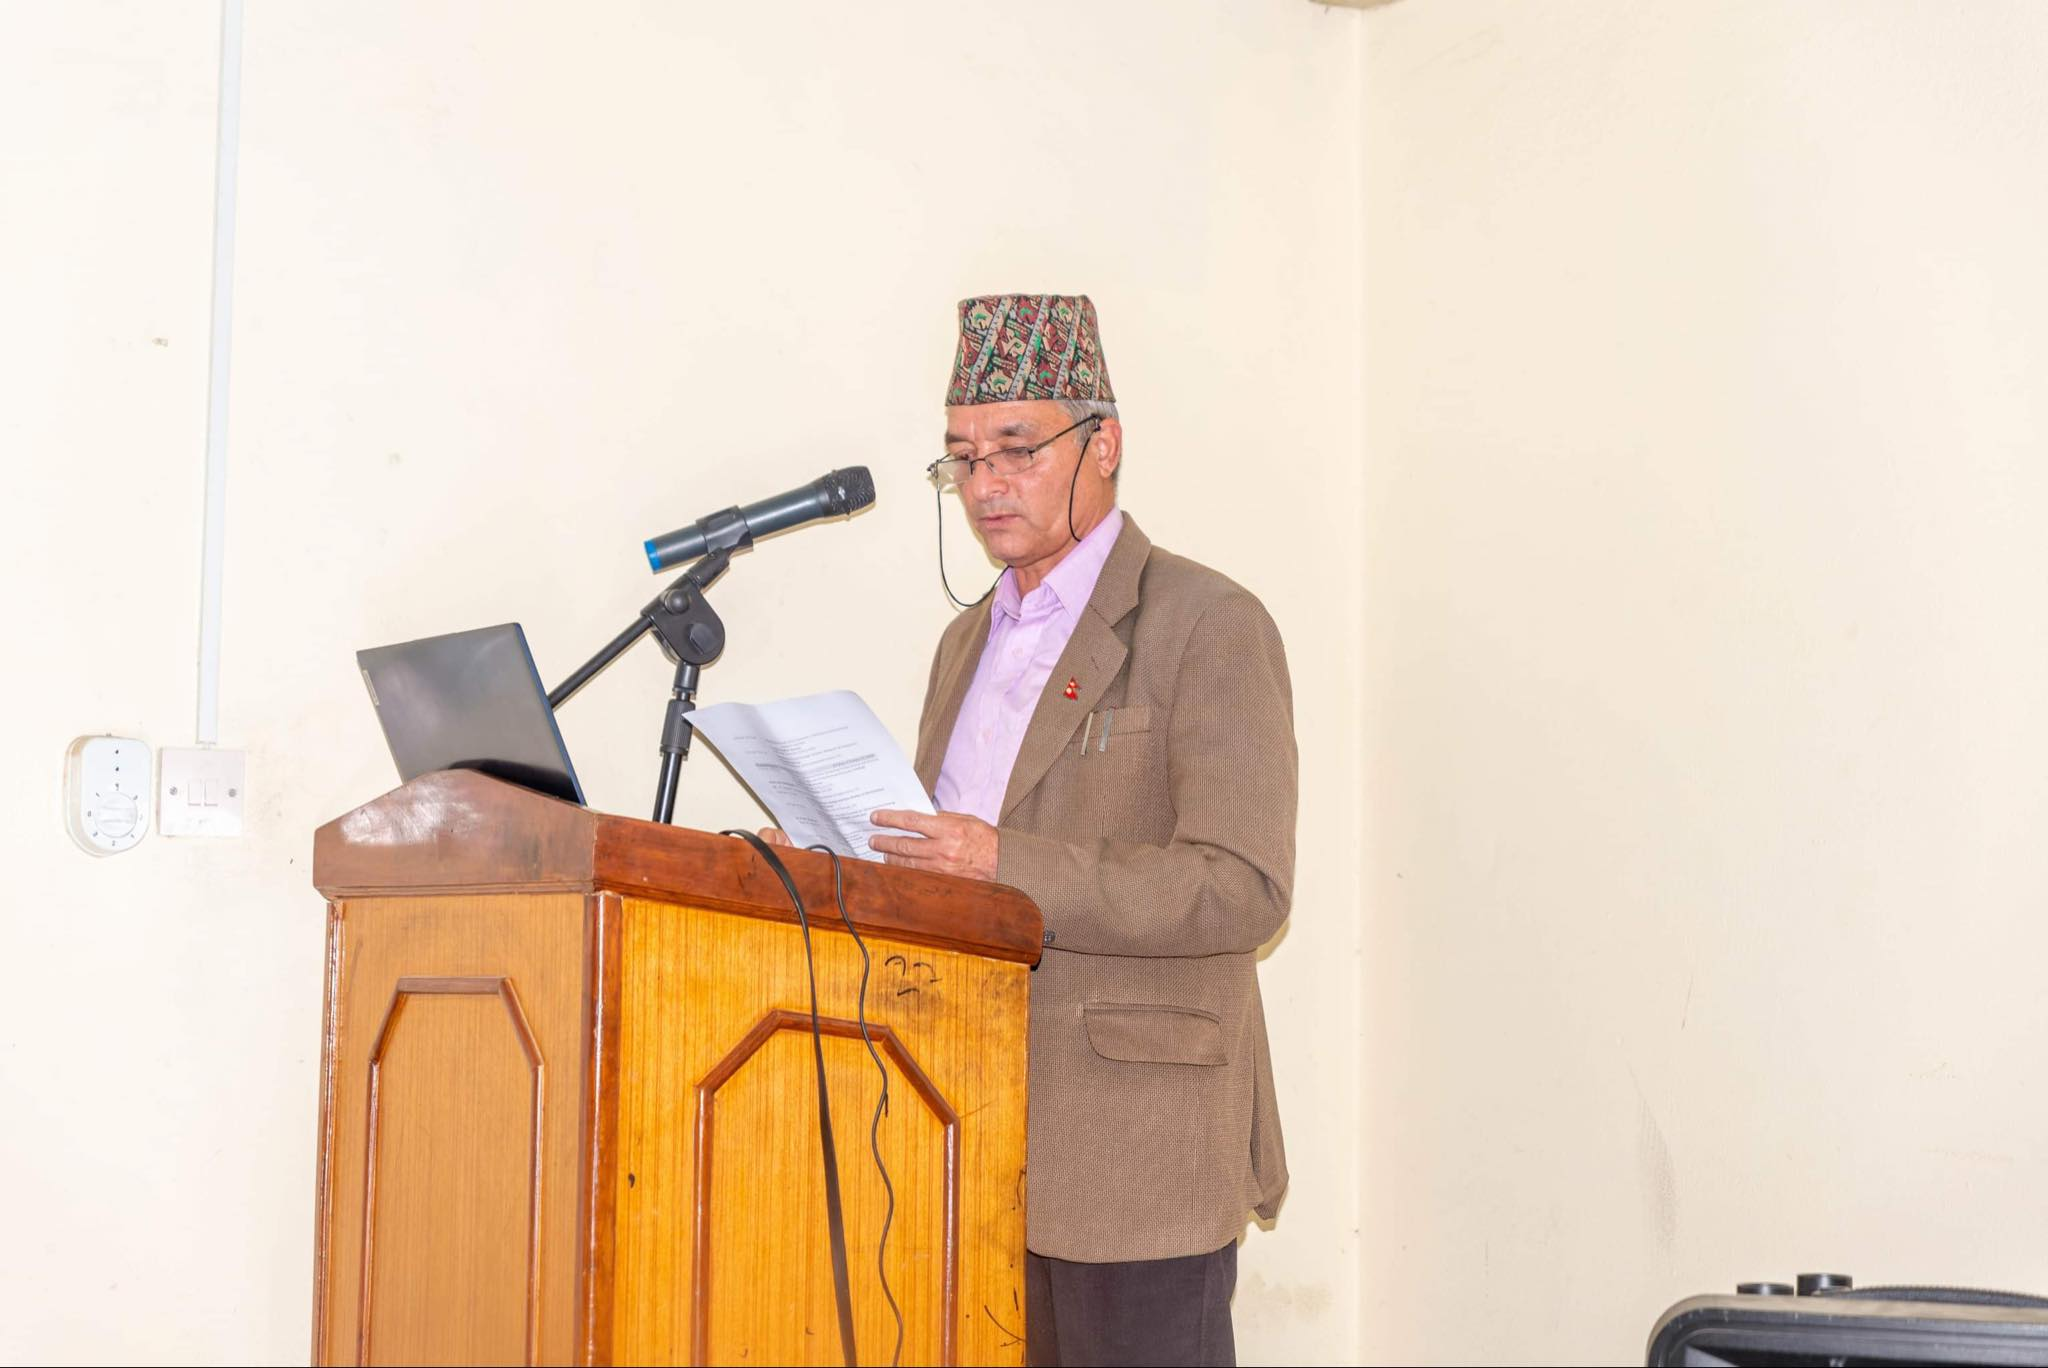
\includegraphics[width=7cm, height=5cm]{chet.jpeg}\\
  \hspace*{5mm}Prof. Dr. Chet Raj Bhatta

  \columnbreak
  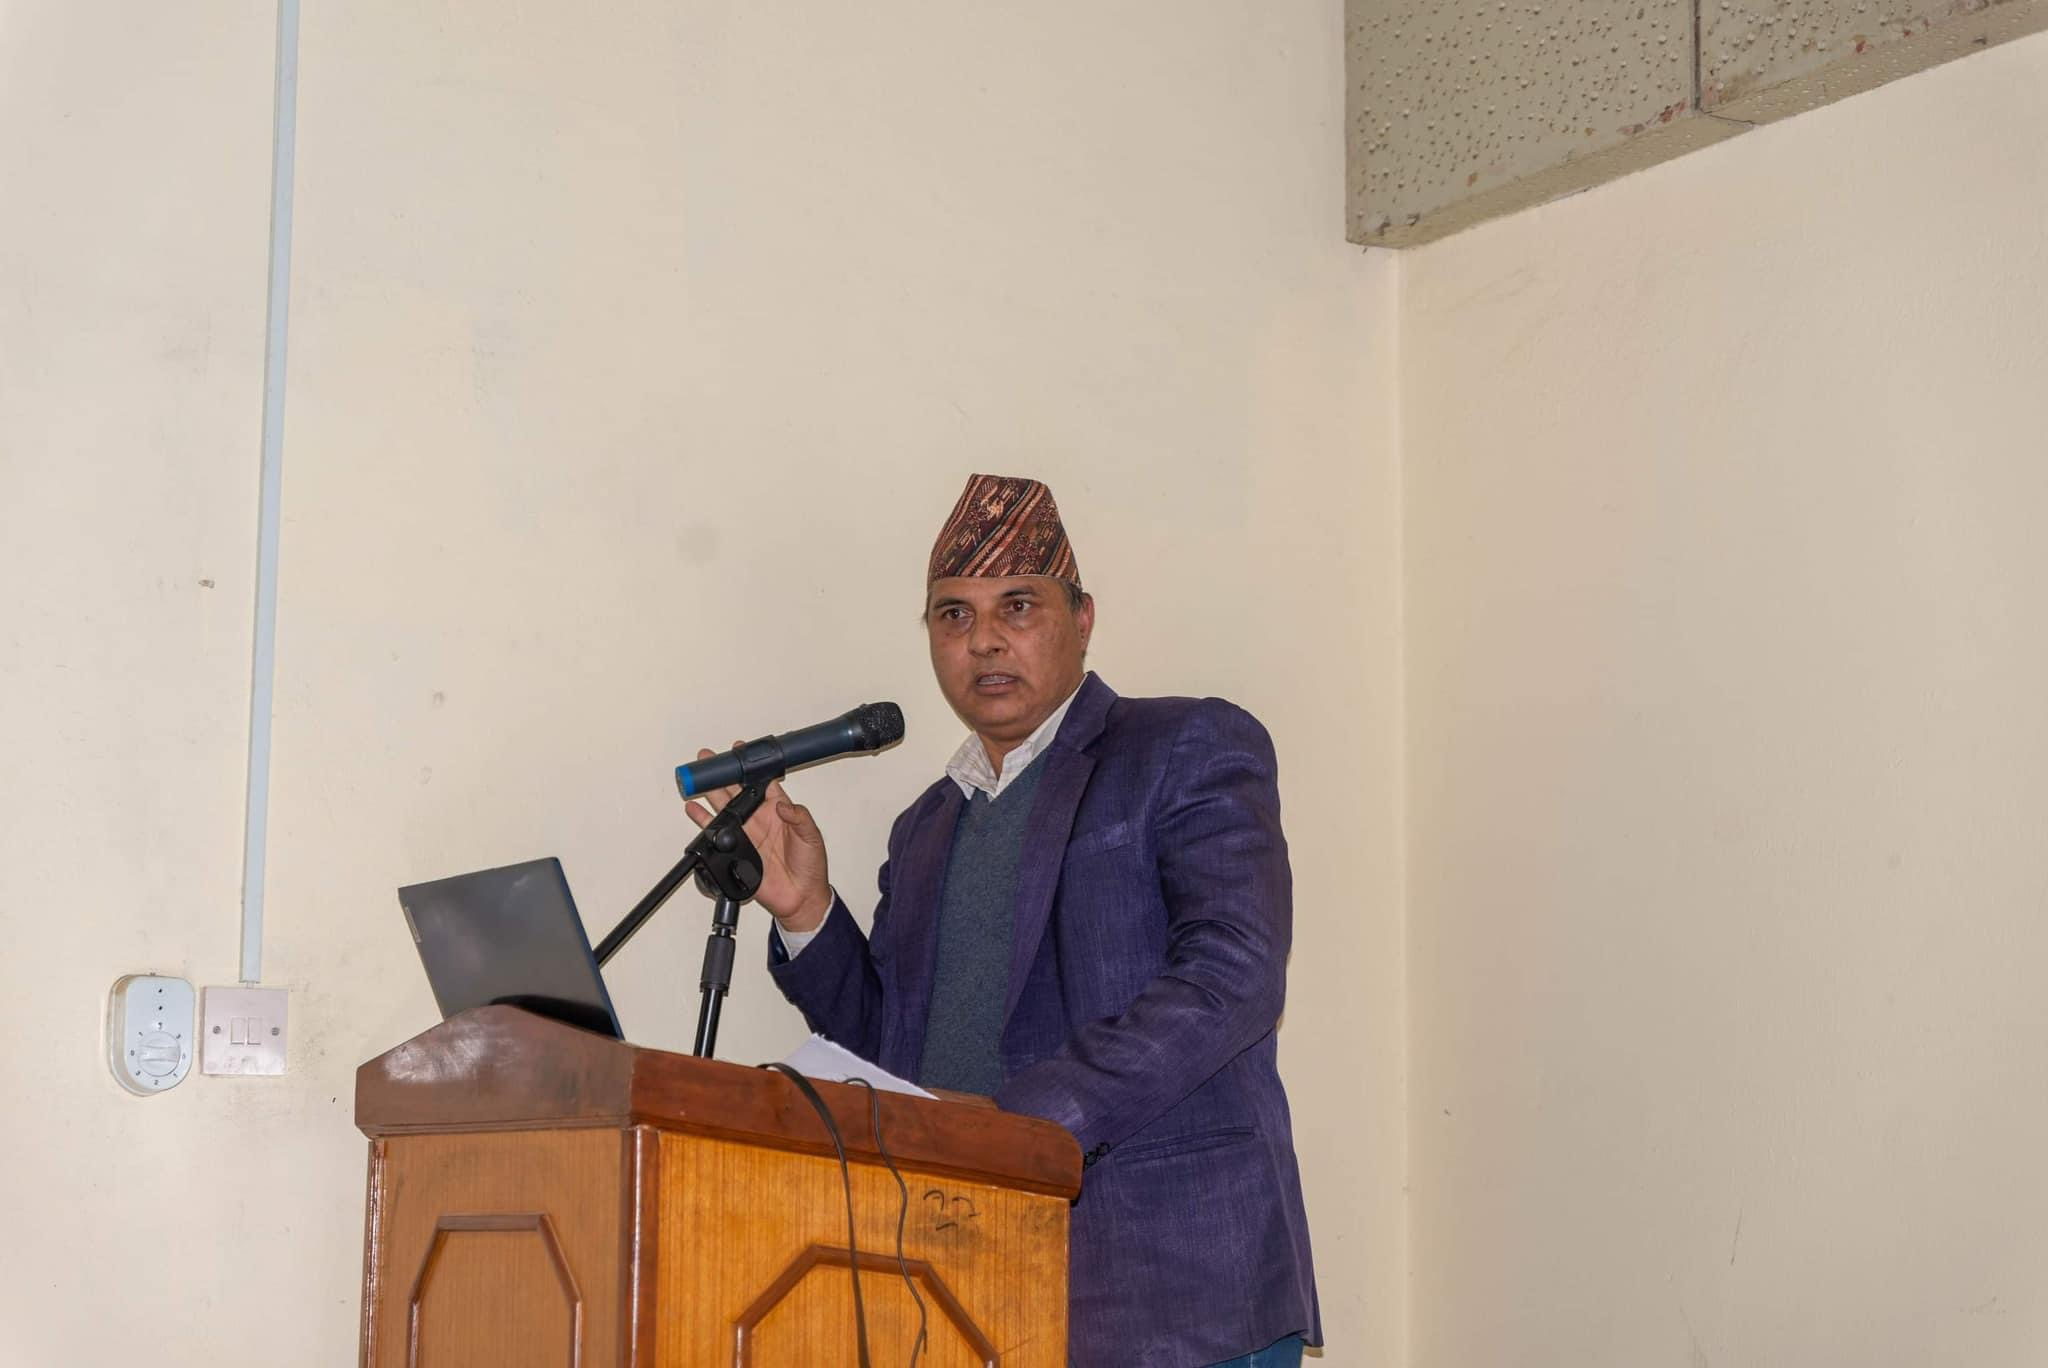
\includegraphics[width=7cm, height=5cm]{np.jpeg}
  \hspace*{3mm} Prof. Dr. Narayan Prasad Pahari
\end{multicols}

\vspace*{5mm}
\noindent
Then the President of Nepal Mathematical Society spoke on the importance of collaborative research and the Chairman of the workshop welcomed everyone to the workshop and give his best wishes. Then other guests also spoke on emerging issues of climate change and responsibilities of the young scientists to solve this issue and gave their best wishes for the success of this workshop.
\clearpage

\begin{center}
  {\bfseries \Large Training Session 1}
\end{center}
\vspace{3mm}

{\bfseries \large Workshop 1}\\[3mm]
The first expert was the Head of the Department of Hydrology and Meteorology, TU Prof. Dr. \textbf{Deepak Aryal}. He gave training on \textbf{Impact of Climate Change on Southern Slope of Himalayan}. He showed that from the study of his team southern slops are more affected by the climate change than the northern slops; snows on the southern slops are melting at an alarming rate. This has adverse effect on the life of Nepal as we are faced to the southern slopes.\\
Then he encouraged young students from the Central Department of Chemistry, TU to come out of the traditional chemistry lab and work on the natural lab of atmosphere where the reactions of chemistry are happening naturally. This new field of subject is atmospheric chemistry which is crucial in studying the phenomenon of climate and climate change.
\vspace{3mm}

\begin{figure}[h!]
  \centering
  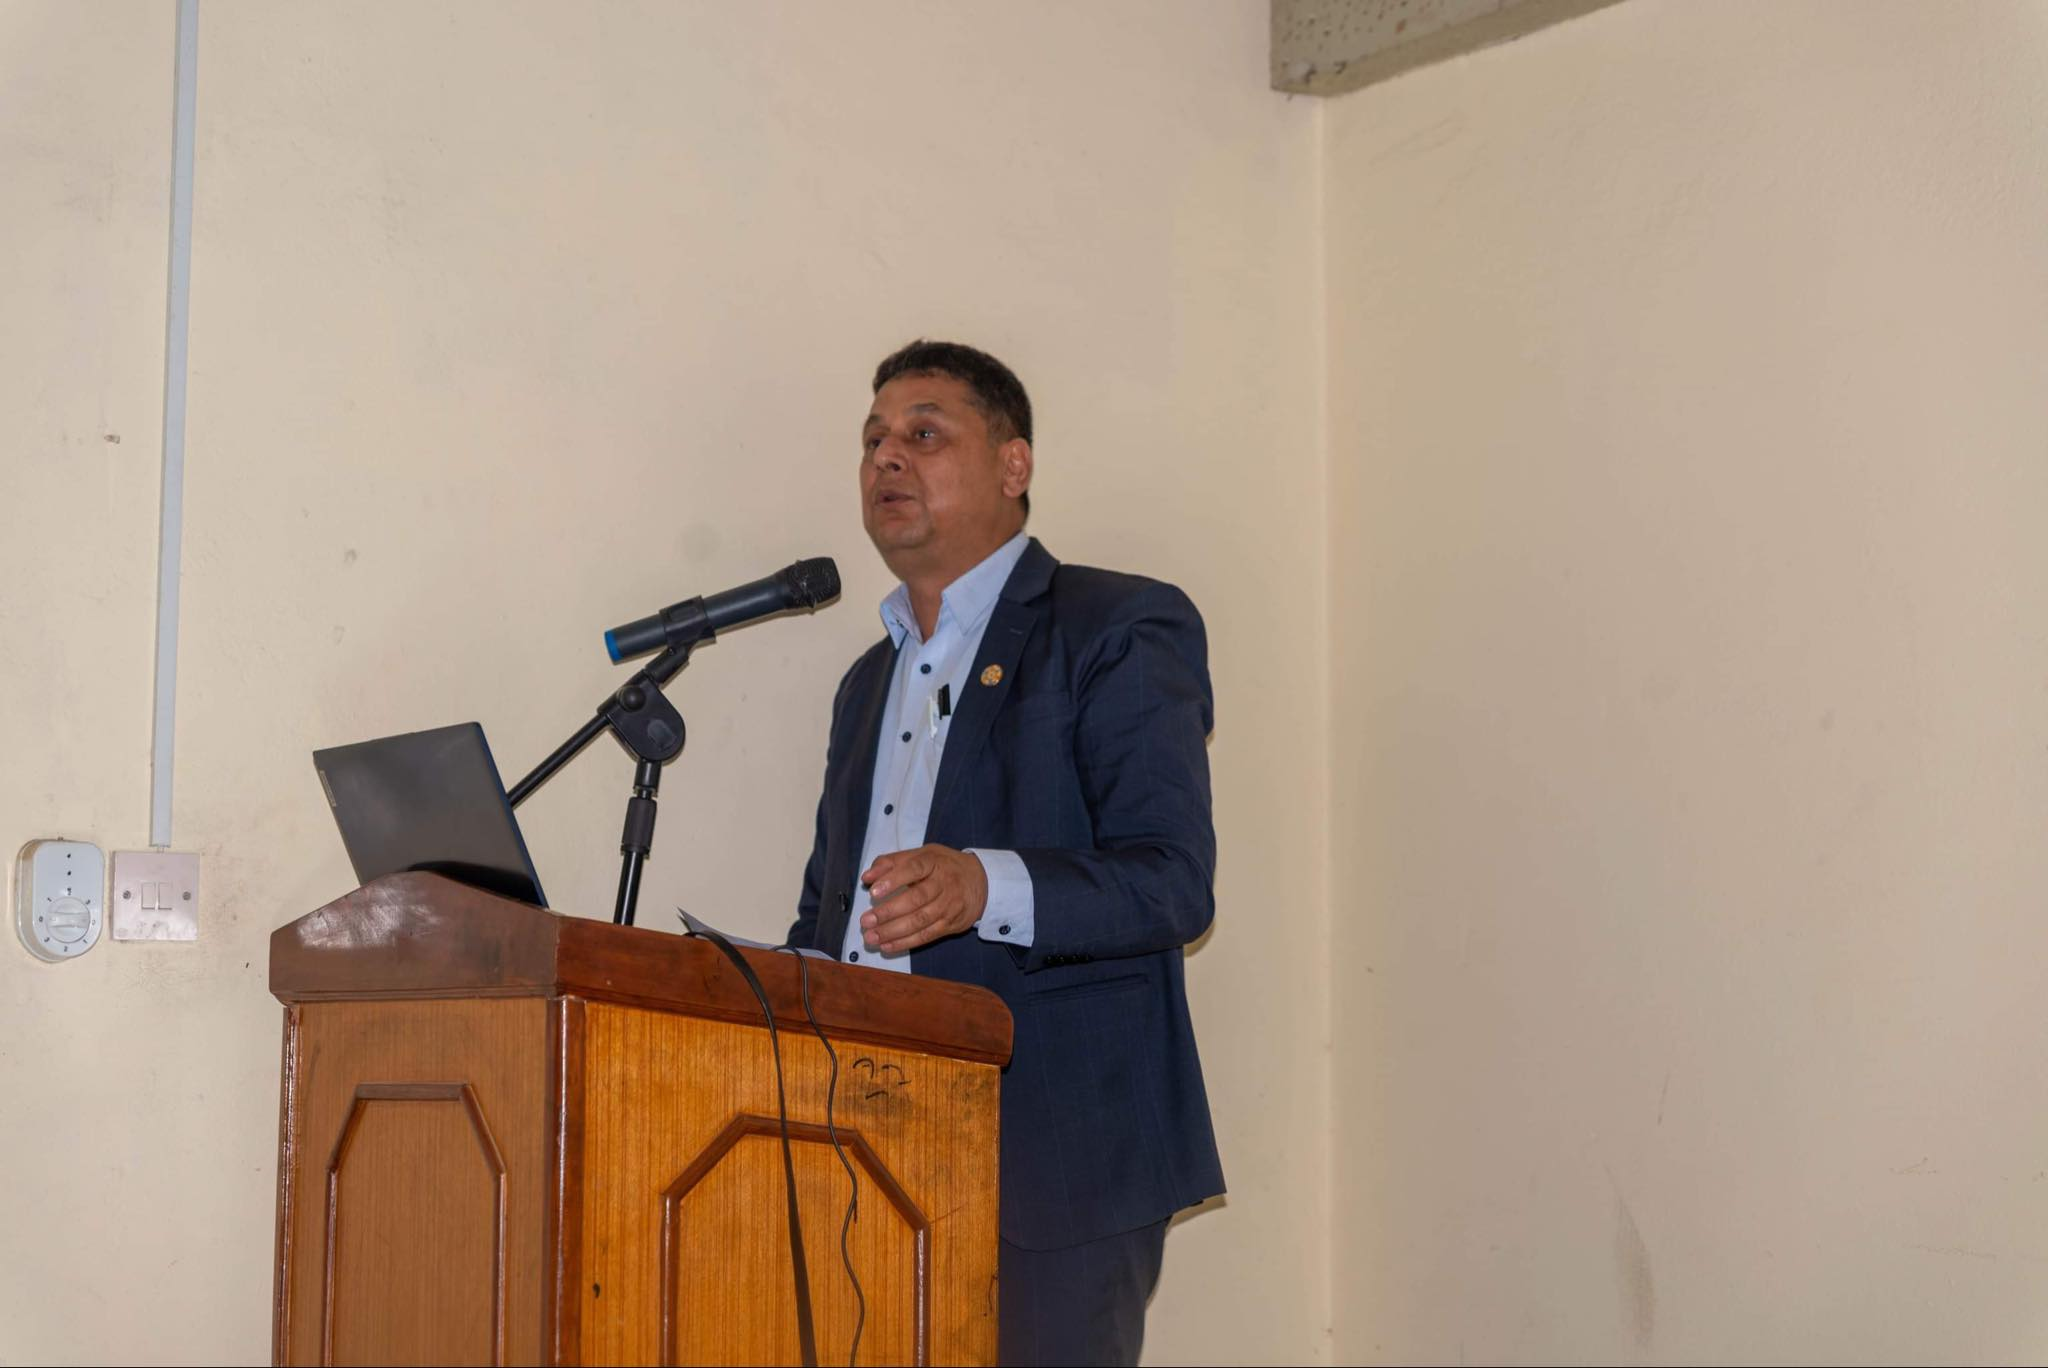
\includegraphics[width=9cm, height=5.7cm]{deepak.jpeg}
  \caption{Dr. Deepak Aryal}
\end{figure}

At 1:30 the session broke for lunch.\\

\vspace{5mm}

{\bfseries \large Workshop 2}\\[3mm]
In this session there was presentations from the \textbf{PhD Students} of Mathematics of Central Department of Mathematics, TU. The Presenters were Mr. Chudamani Pokharel, Mr. Pushpa Nidi Gautam, Mr. Bekha Ratna Dangol, Mr. Chet Nath Tiwari and Mr. Shankar Pariyar.\\[3mm]
Mr. Pokharel presented on \textit{Analysis of Blood Flow through Stenosed Artery with Einstein Viscosity}, Mr. Gautam presented on \textit{Blood Flow through a Curved Stenotic Artery}, Mr. Dangol presented on \textit{Complex Granular Slides and Flow-Obstacle-Interaction}, Mr. Tiwari presented on \textit{Novel Mathematical Models for Impact Pressure and Mobilization Length} and Mr. Pariyar presented on \textit{Fractional Advection Diffusion Equations in Caputo-Fabrizio Sense}.
\clearpage

{\bfseries \large Workshop 3}\\[3mm]
The expert of session was \textbf{Dr. Rameshraj Pant} of Central Department of Environmental Science, TU. He gave training on Impact of Climate Change in Nepal and its Mitigation and Adaptation. His talk was very descriptive and informative. His conclusion was that the climate change has very adverse effect in Nepal. It has affected our agriculture, our weather and our overall life style. Heavy rain in summer and drought in winter and the change in vegetation and habitats of wild animals are among the effects.
\vspace{5mm}

\begin{figure}[h!]
  \centering
  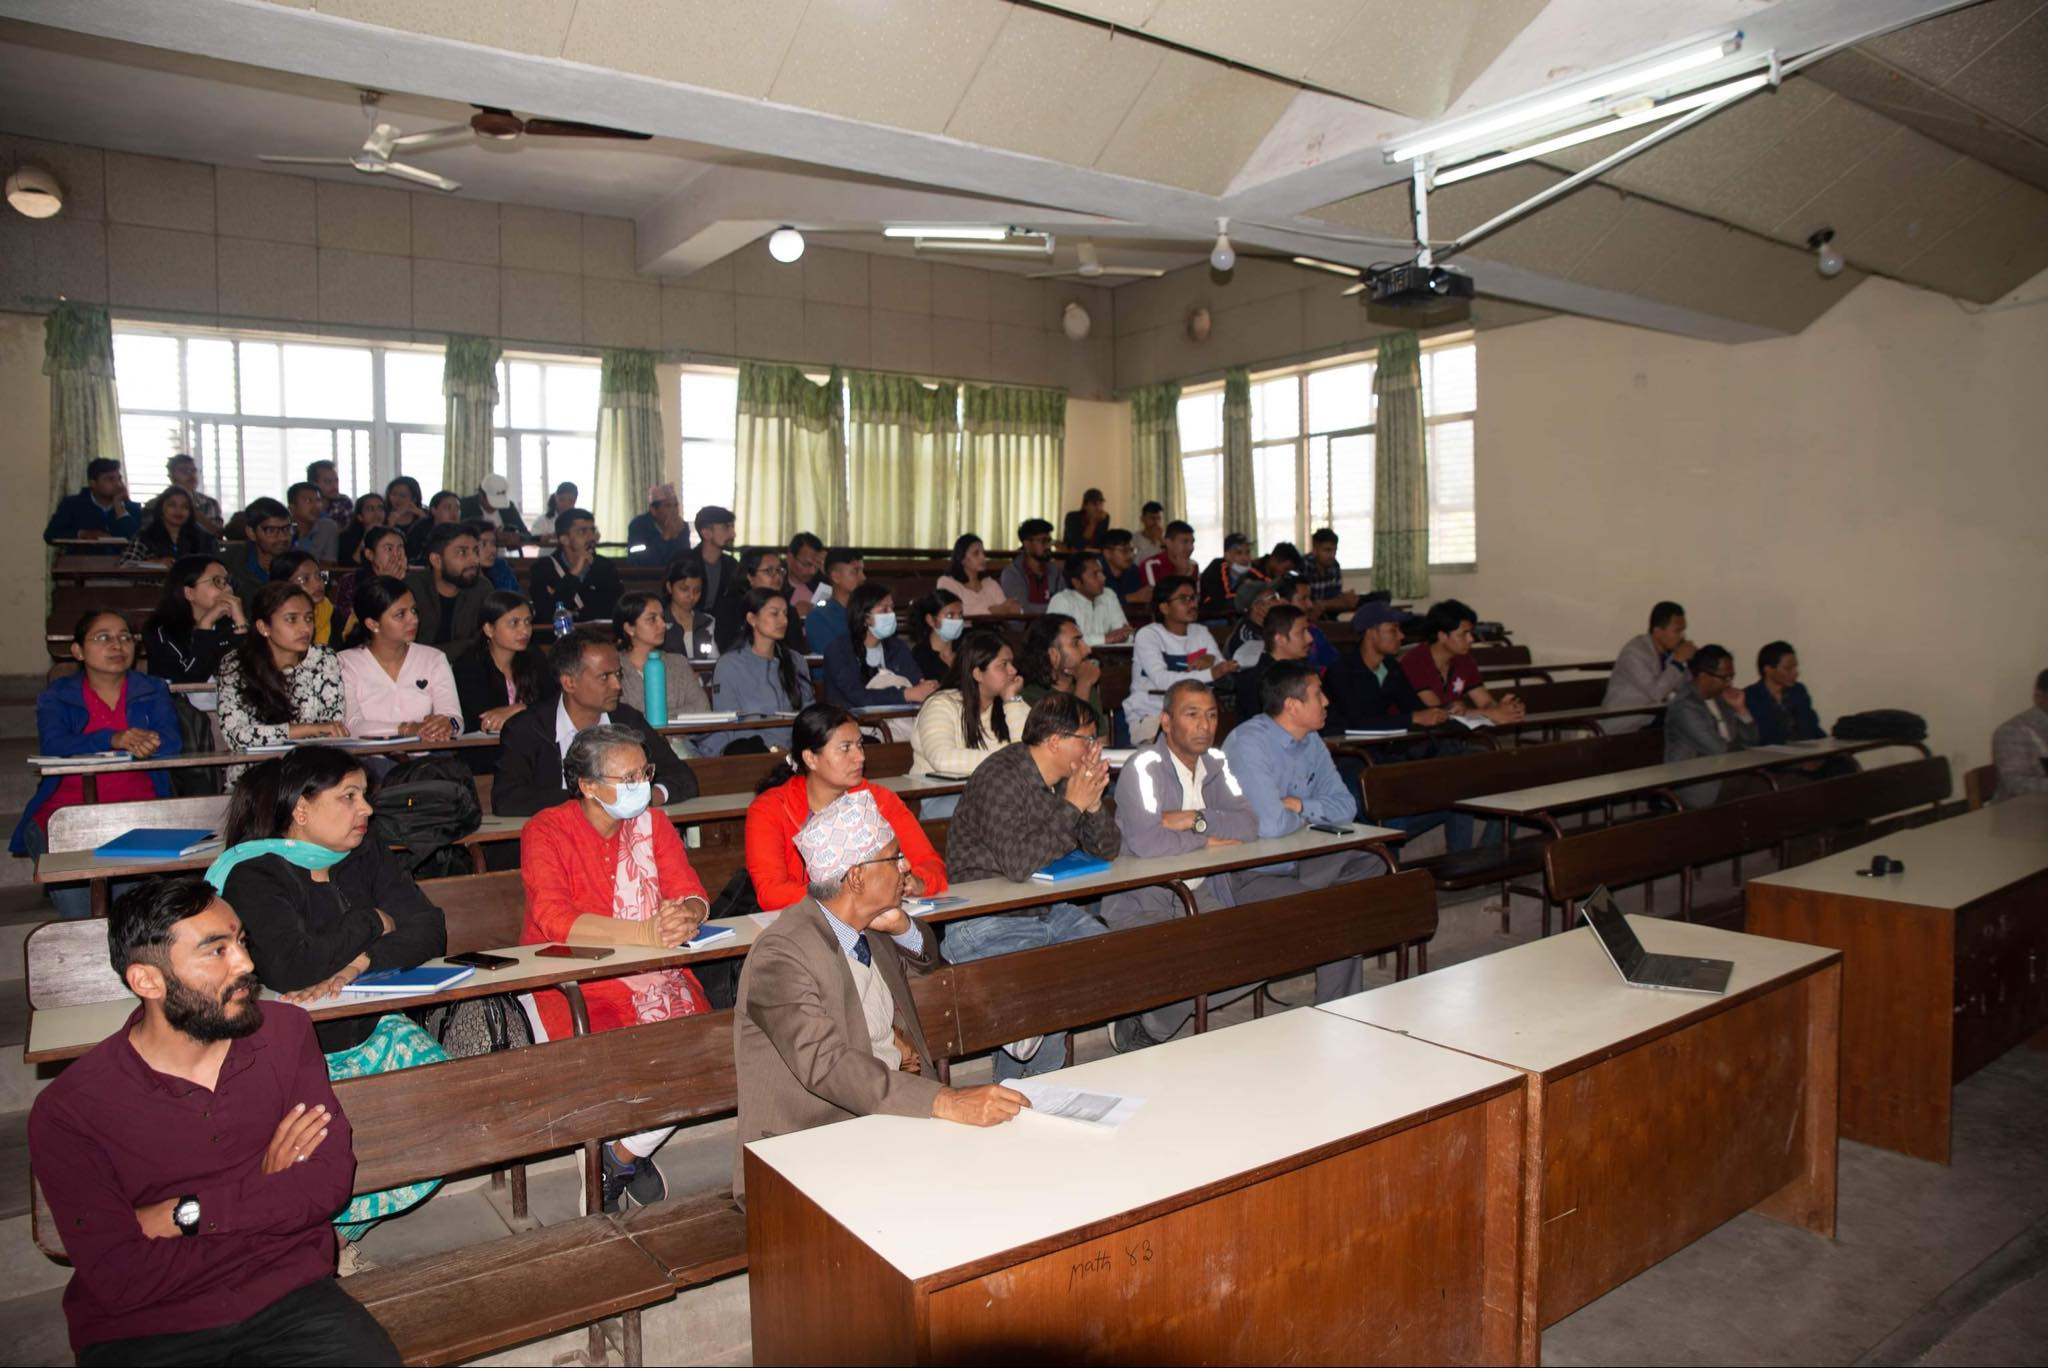
\includegraphics[width=13cm, height=8cm]{ss.jpeg}
\end{figure}

\vspace{10mm}

\begin{figure}[h!]
  \centering
  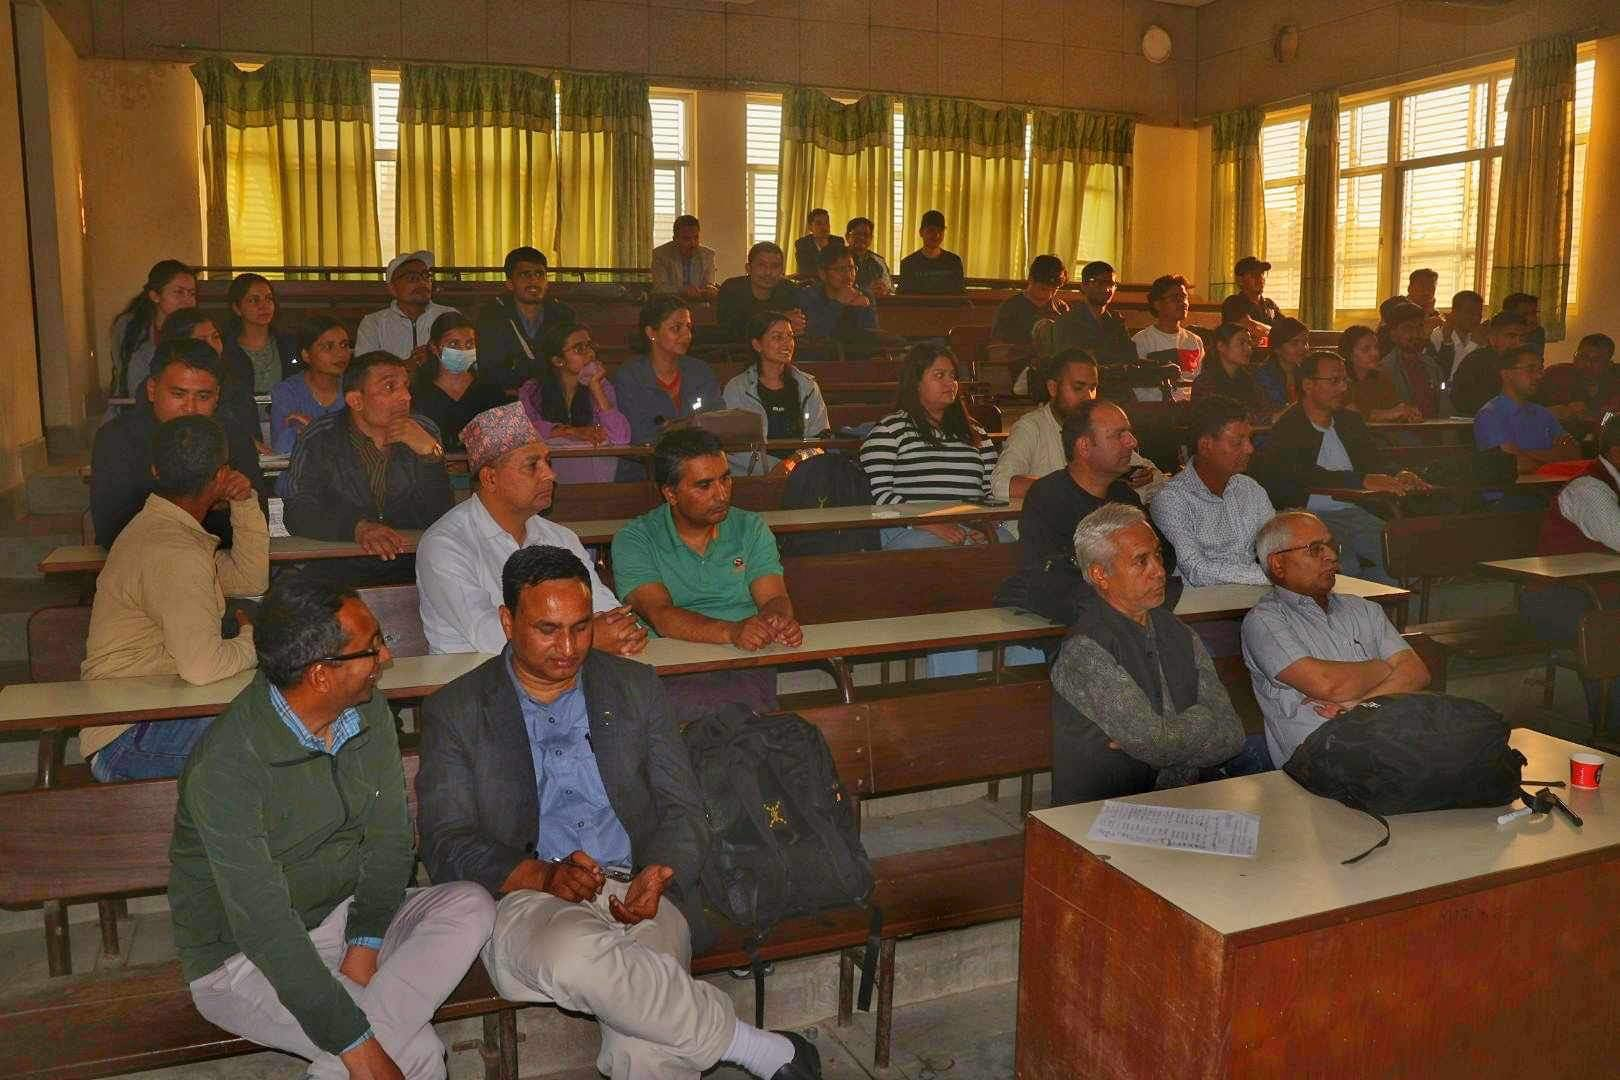
\includegraphics[width=13cm, height=8cm]{r.jpeg}
\end{figure}
\clearpage

\begin{center}
  {\bfseries \Large Training Session 2}
\end{center}
\vspace{5mm}

{\bfseries \large Workshop 4 : Online Session}\\[3mm]
The expert of the online session was \textbf{Dr. Madhav Ghimire} of Central Department of Physics, TU who gave the training via zoom-meeting. This session was open to everyone and most participants were from physics department.\\[3mm]
The training Dr. Ghimire gave was on how to use \textbf{super computer} of Tribhuvan University. Artificial Intelligent, Deep Learning, Data Analysis, are crucial tools in modern research. The predictions and forecast of weather is not possible without use of these tools and these tools needs a super computer. In fact any heavy data based research needs a super computer. He also show-cased the research done by his team in sold physics to the participants.

\vspace{2cm}

{\bfseries \large Workshop 5}\\[3mm]
The expert of this session was Head of Central Department of Geology, TU Dr. \textbf{Dinesh Pathak}. He gave training on \textit{Climate change and Geo-disaster in the Himalaya}. The relation between climate change and geo-disaster was discussed. He then trained on evacuation and safety measures during disasters. He then show-cased the effect of climate change on various geological terrains of Nepal. He also talked on publishing research articles in Journals.

\vspace{4mm}
\begin{figure}[h!]
  \centering
  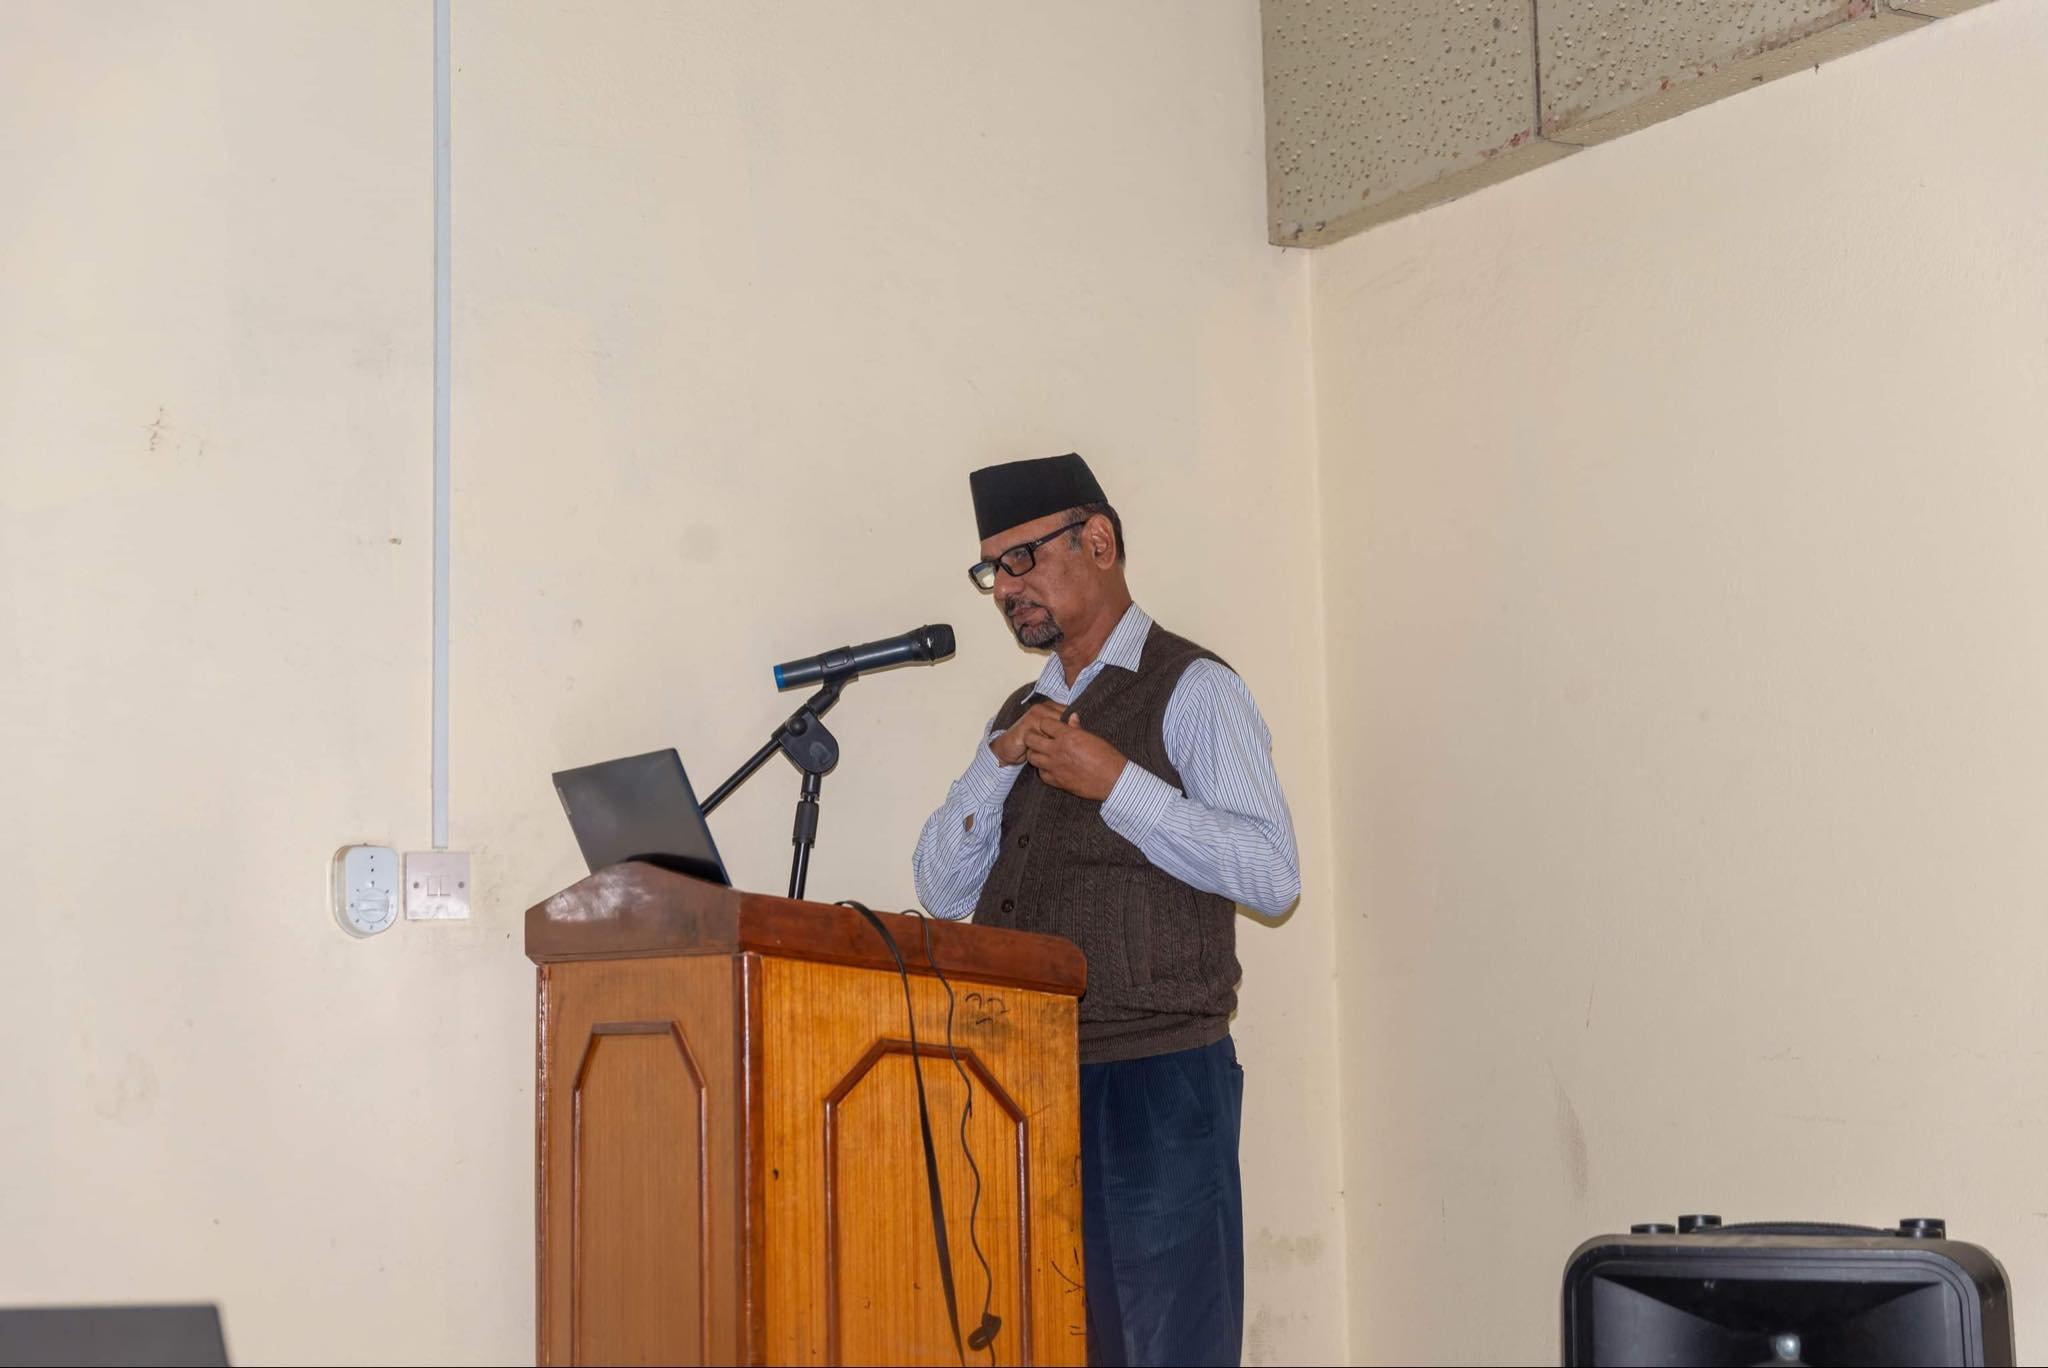
\includegraphics[width=10cm, height=7cm]{pathak.jpeg}
  \caption{Dr. Dinesh Pathak}
\end{figure}
\clearpage

{\bfseries \large Workshop 6}\\[3mm]
The expert of this session was Dr. \textbf{Binod Pokharel} of Central Department of Hydrology and Meteorology. He gave training on \textit{Nepal's Climate Conundrum: Dissecting the Evolving Extremes and Changing Climatic Landscape}. He trained the participants on the gobal warming and its effects on rainfall of Nepal. The effect is that winters are getting dryer and summers are getting wetter which has result drought in recent winters in Nepal and heavy rainfall in recent summers in Nepal. His training was based on a \textbf{mathematical model} which used exponential function. The water vapour holding capacity of atmosphere exponentially increases with the increase in temperature.
\vspace{5mm}

\begin{figure}[h!]
  \centering
  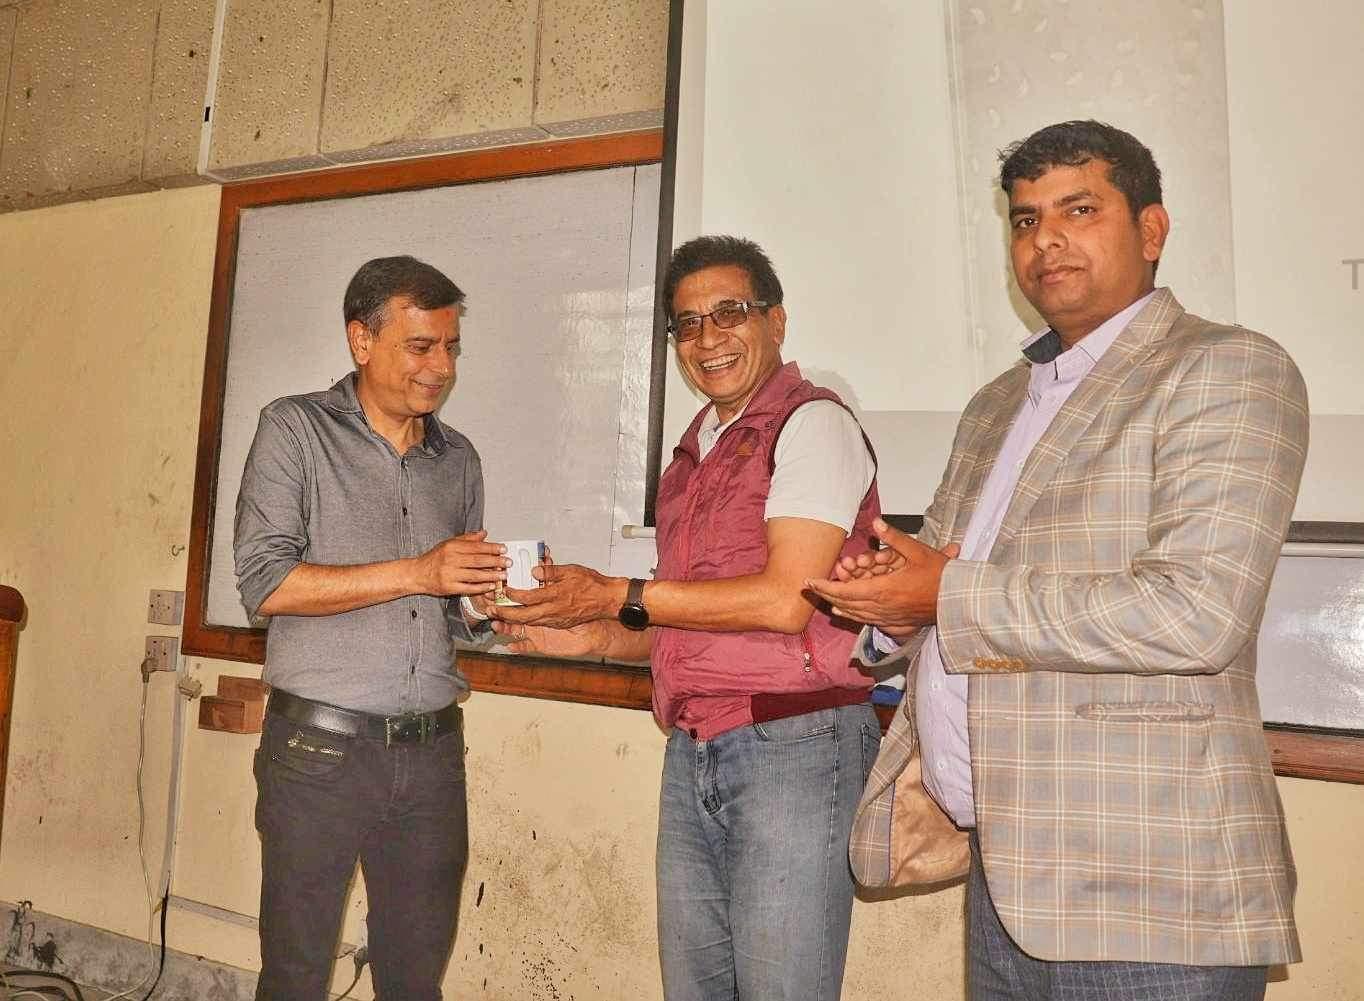
\includegraphics[width=12cm, height=7.5cm]{binod.jpeg}
  \caption{Dr. Binod Pokharel receiving token of love}
\end{figure}

\vspace{7mm}

At 1:30 noon the session broke for lunch.
\vspace{5mm}

\begin{figure}[h!]
  \centering
  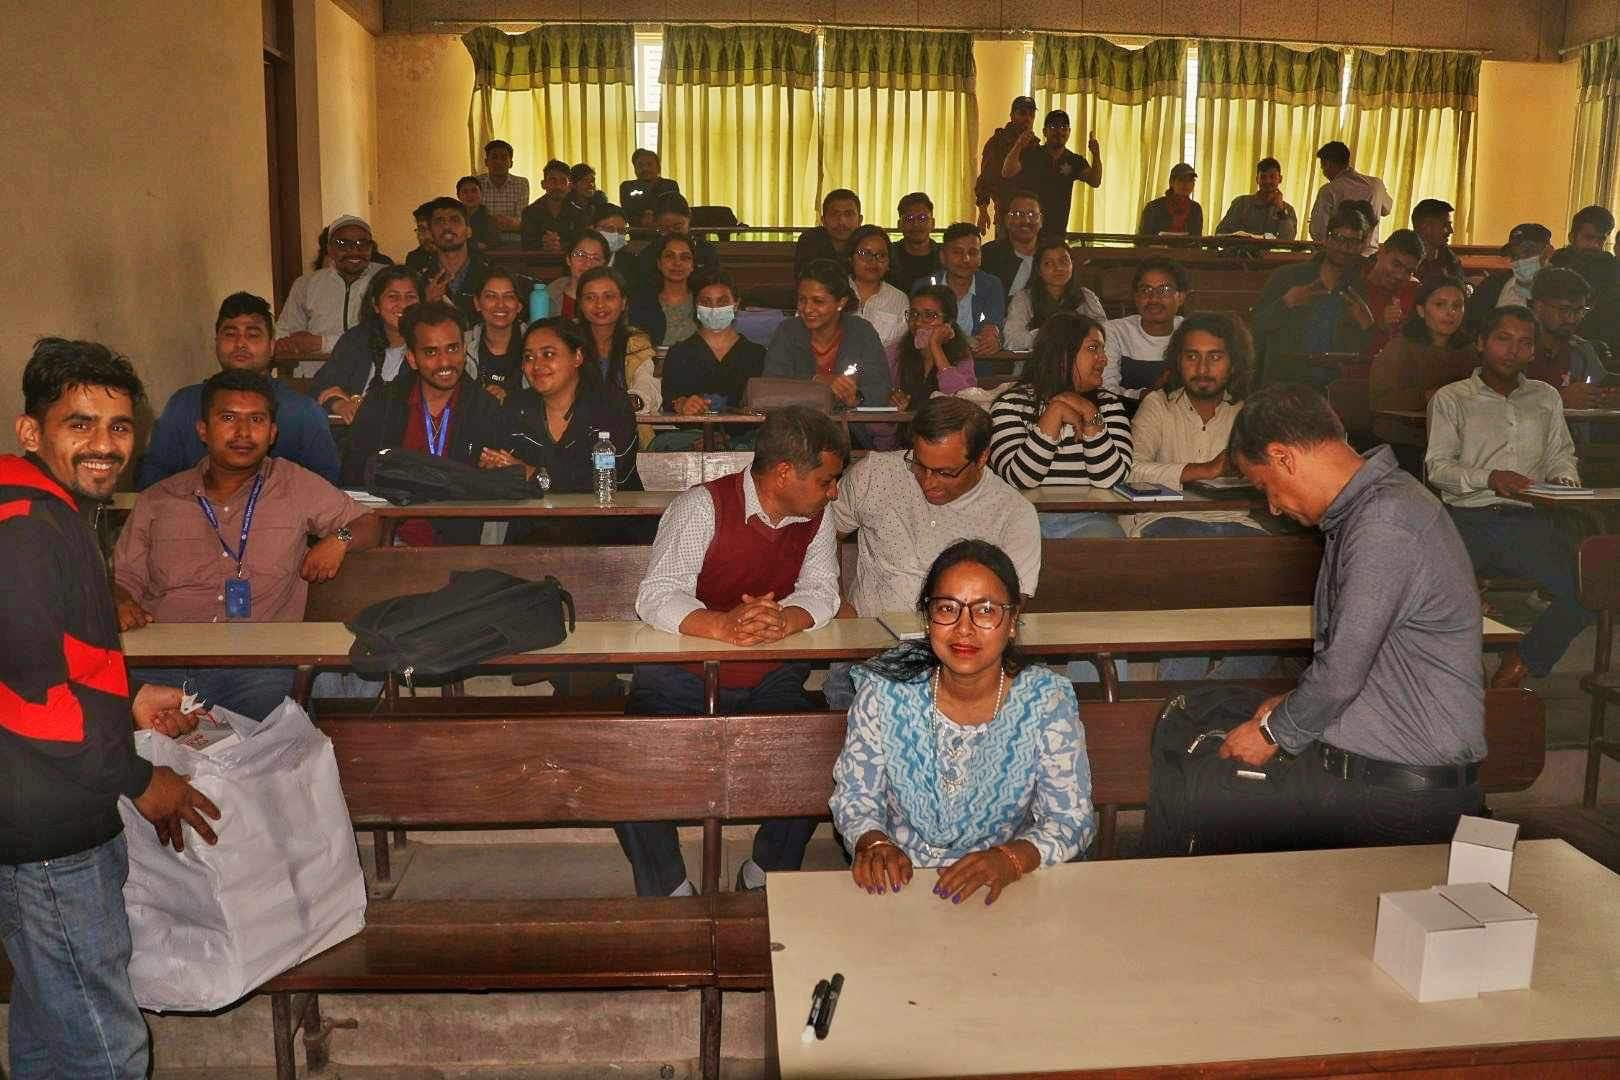
\includegraphics[width=13cm, height=7.5cm]{lunch1.jpeg}
\end{figure}
\clearpage

{\bfseries \large Workshop 7}\\[3mm]
The expert of this session was Dr. \textbf{Bhanu Bhakta Neupane} Central Department of Chemistry, TU. He gave training on \textbf{A nexus between climate change and microplastic}. Microplastics are plastic particles of a very small size. They are emerging issue of today's polluted world. These inorganic particles have adverse effects on both health of biological beings and on climate change.

\vspace{10mm}
\begin{figure}[h!]
  \centering
  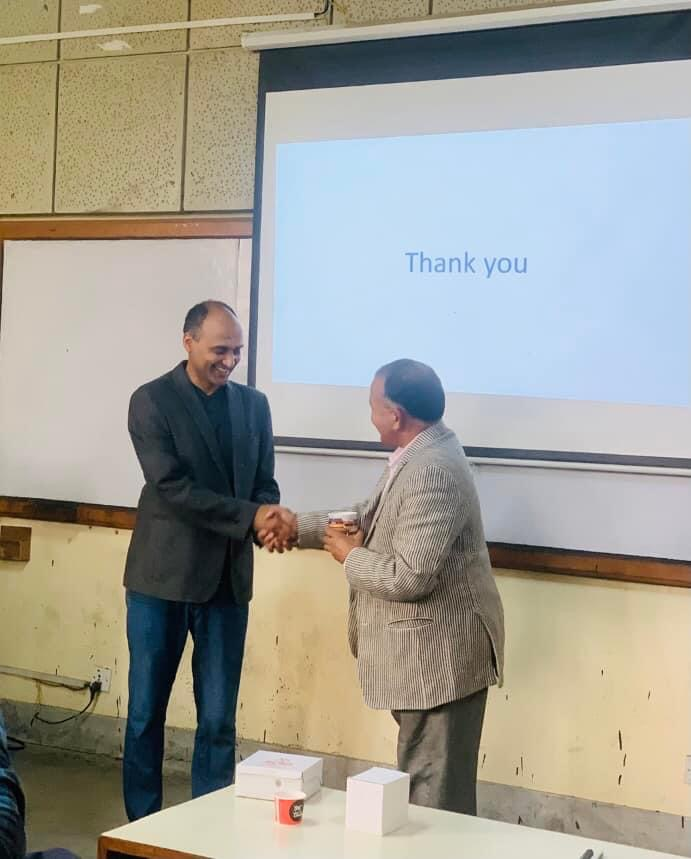
\includegraphics[width=10cm, height=7cm]{neupane.jpeg}
  \caption{Dr. Neupane receiving token love}
\end{figure}

\vspace{23mm}

{\bfseries \large Workshop 8}\\[3mm]
This session was the \textit{CDM alumni talk series} by the former Head of Central Department of Mathematics Prof. Dr. \textbf{Kedar Nath Upreti}. The topic of the talk was Research in \textbf{Mathematics and Its Exposure}.\\[3mm]
He discussed the methods and ways of doing an academic research. An academic research is generally a thesis writing or an article writing which is a challenging job. It requires time and knowledge and hard-work of the researcher. Generally it starts with a selection of a supervisor and a topic of research.Then he discussed the methods of publishing research papers and challenges faced during publication. Finally he discussed the issue of plagiarism in research papers which is a serious issue.
\clearpage

\begin{center}
  {\bfseries \Large Closing Session}
\end{center}
\vspace{5mm}

{\bfseries \large Remarks by the Participants}\\[3mm]
There participants from three different departments came forward to give their remarks on the workshop. First Mr. \textbf{Aditya Adhikari} of Central Department of Mathematics, TU remarked that the workshop was successful in promoting collaborative research and interdisciplinary research. Second \textbf{Dinesh Raj Regmi} of Central Department of Geology remarked that this workshop was helpful in bring researchers from different background together in discussing the common issue of climate change and such programs should be conducted frequently. Third Ms. \textbf{Saraswoti Pokhrel} of Central Department of Chemistry, TU remarked that the workshop had met her and her friends all expectations except they expected more training than talks on the workshop. Other than that, they had a great time and would look forward to such events organized by the Central Department of Mathematics.\\[5mm]

{\bfseries \large Remarks by the President of CDM Student Council}\\
The President Mr. Sandesh Thakuri thanked Dr. Kafle and Dr. Bhatta for organizing such a historic event. He said,
\begin{figure}[h!]
  \centering
  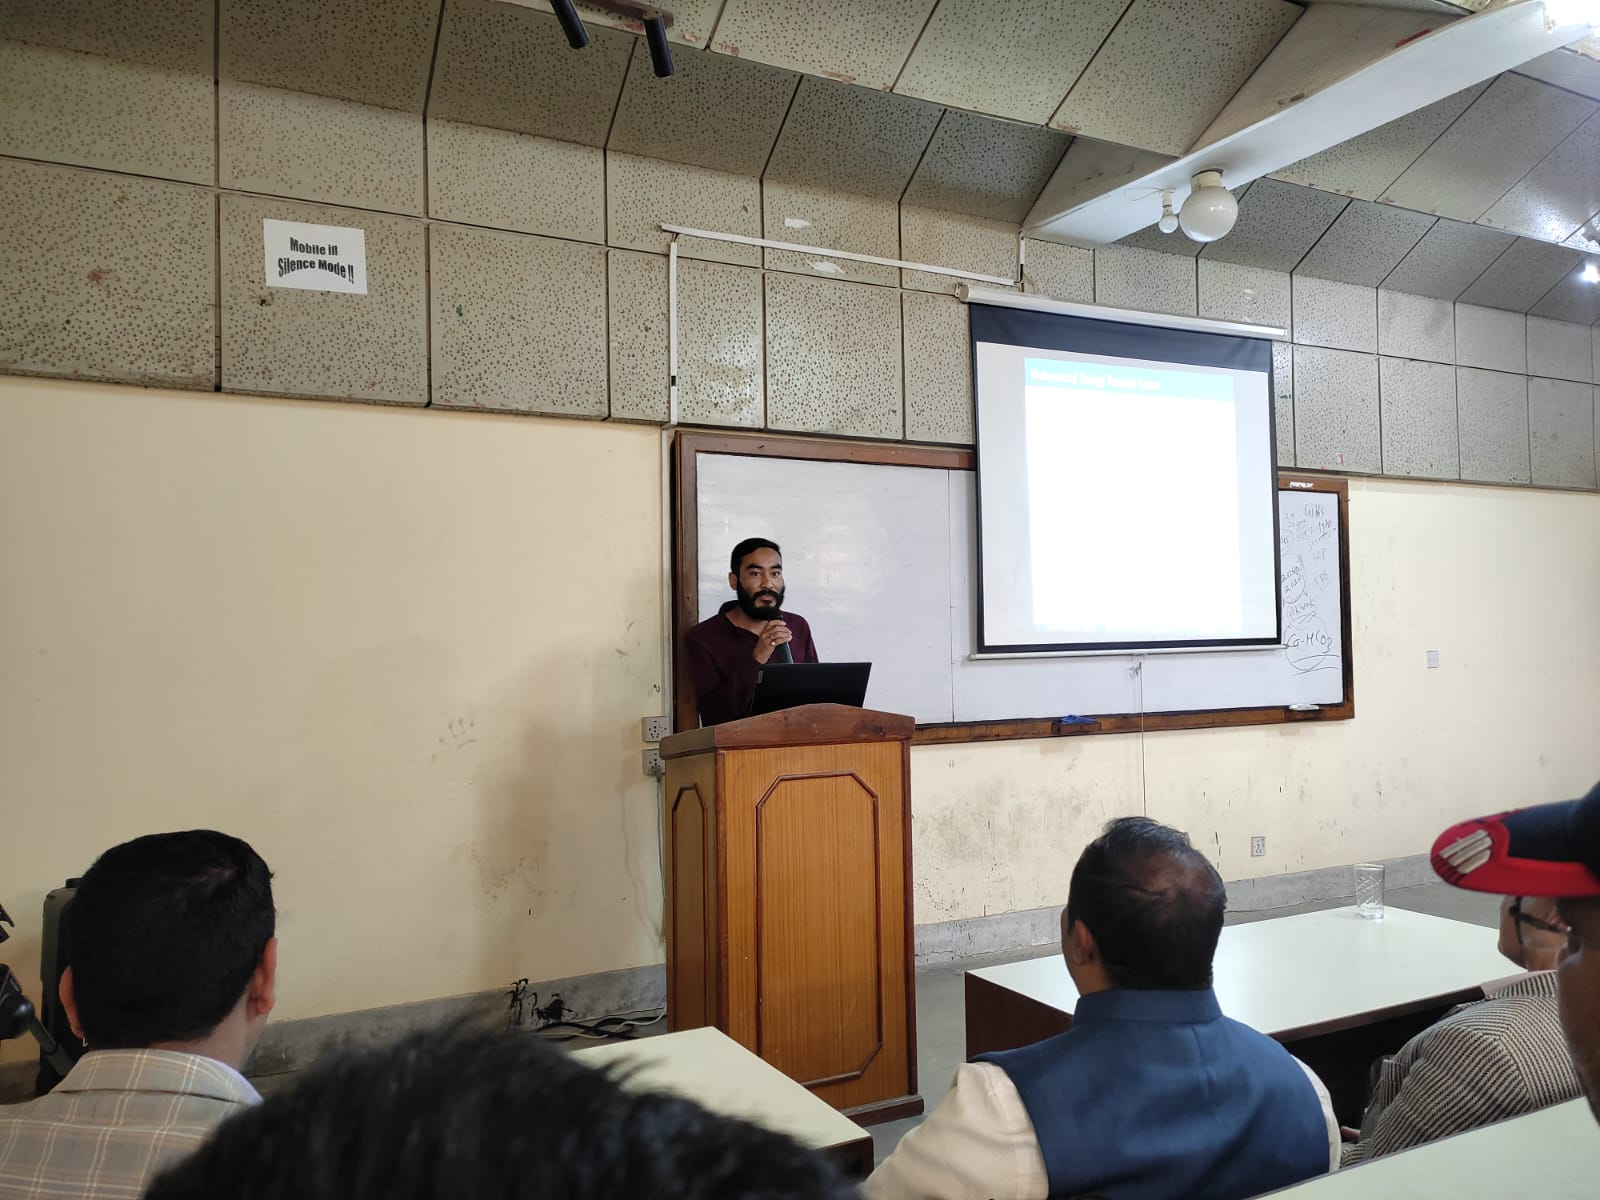
\includegraphics[width=12cm, height=7cm]{president.jpg}
\end{figure}
\vspace{3mm}
"We had to come together but hadn't found a convincing issue to do so. Climate Change seems to be the general issue that has brought us all together here. It has been my own wish for a very long time to bring all the departments of TU under the same roof of mathematics. Mathematics can the that unifying agent as it is universal and general. Mathematics needs every subject and every subject needs mathematics. It seems climate change and all the issue of modern world needs a general solution a solution from every sector, which demands a strong collaboration. A complete solution is not possible without a strong collaboration. \textbf{Mathematics can be that glue of that collaboration}.
\clearpage

The departments of TU are very close interms of distance but very far interms of collaboration. This distance needs to be shortened and removed. Every kinds of research is being done in Central Department of Mathematics; research about blood, about evacuation, ... Research on same topics are also being done in the respective departments.
"\\
Then he gave a big thank you to the Council for working so hard to make this workshop successful.\\[7mm]

{\bfseries \large Concluding Remarks}\\[3mm]
Then Dr. Ramesh Raj Pant and Vice President of Nepal Mathematical Society
Dr. Shree Ram Khadka give their remarks about the workshop. Finally the workshop was concluded by the chairman of the workshop Head of Central Department of Mathematics, TU Prof. Dr. Chet Raj Bhatta by declaring the success of the workshop and giving a big thank you to the organizing team.\\[3mm]

{\bfseries \large News and Reports}\\[3mm]
The news of the workshop was covered by the two national online news portals. The first day of the workshop was covered by the \textbf{Bygankhabar} media: \href{https://bigyankhabar.com/news/466?fbclid=IwZXh0bgNhZW0CMTEAAR2T6N0ZWHThH36HAoFJzrOioSew3a5q9cheBVtr23fTcmynHWW23u9kL7Q_aem_Ab1AITgAqW20AfXdGEopIJzsS-SPnux6ygiMfDMx6DCzY9p1xqf0KG2THdmgxjEKleYf9EwSC_gBVom8hVjHb8Y1}{News Link1}.\\
The second day of the workshop was covered by the \textbf{Boudhakhabar} media:
\href{https://www.boudhakhabar.com/details/5789?fbclid=IwAR3h4kfiercOQEBUr2oSNwfA1fBK4yhx0DEQxMiiGN-5kWbVKvWYWtkgyrw}{News Link2}\\[4mm]

{\bfseries \large Certificate Distribution Clips}\\[3mm]
 \begin{figure}[h!]
  \centering
  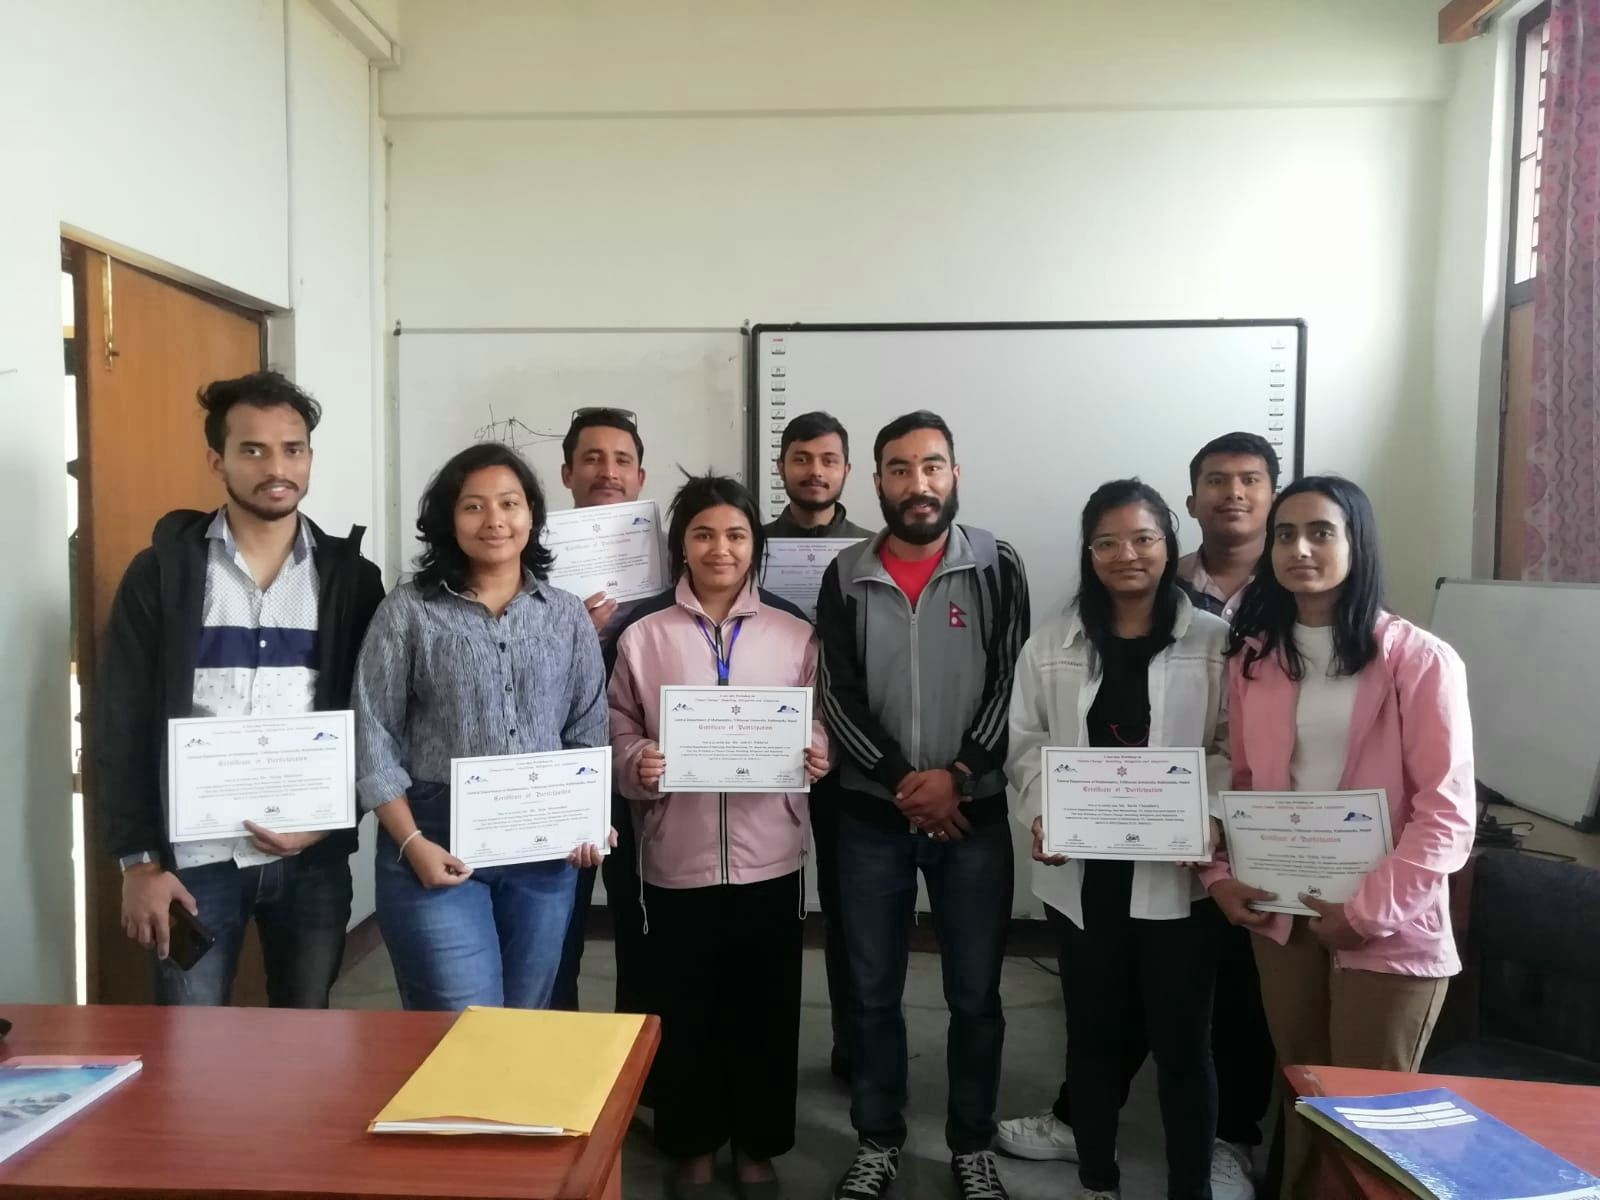
\includegraphics[width=12cm, height=8cm]{certificate.jpg}
  \caption{\small At Central Department of Hydrology and Meteorology}
\end{figure}
\clearpage

{\bfseries \large List of registered Participants}
\begin{figure}[h!]
  \centering
  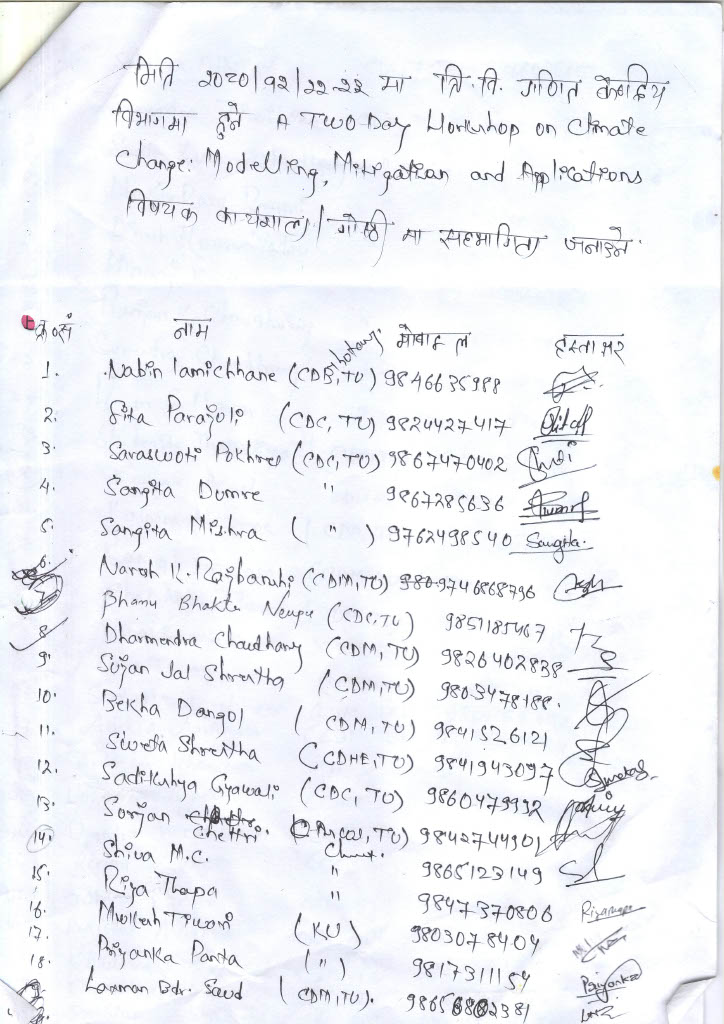
\includegraphics[width=12cm, height=12cm]{1.jpg}
  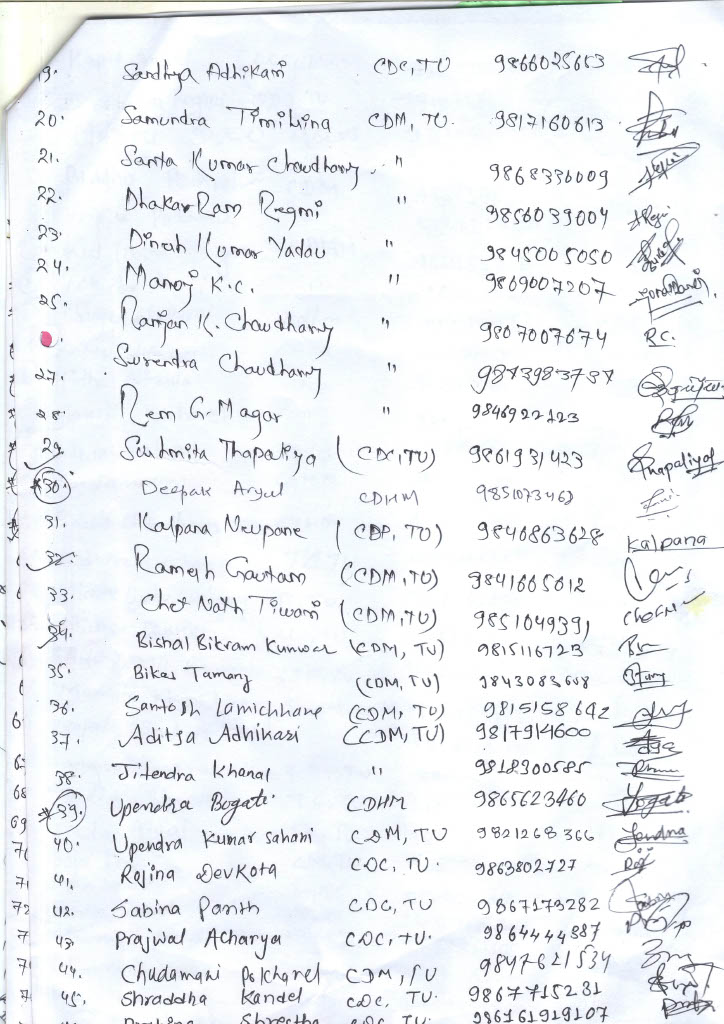
\includegraphics[width=12cm, height=12cm]{2.jpg}
\end{figure}

\begin{figure}[h!]
  \centering
  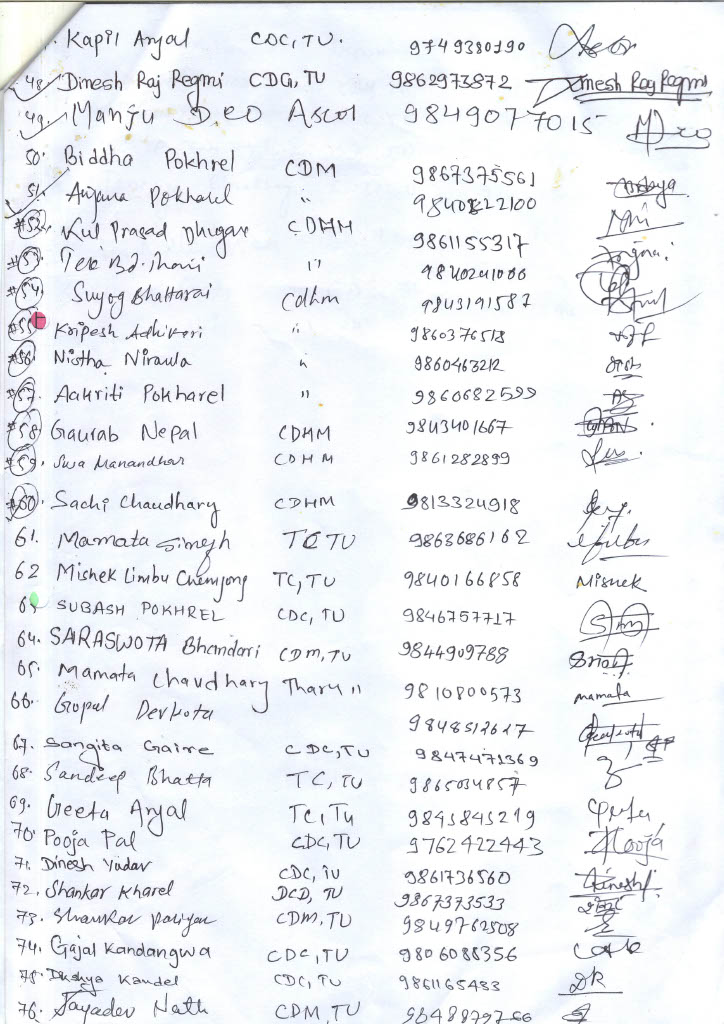
\includegraphics[width=12cm, height=12cm]{3.jpg}
  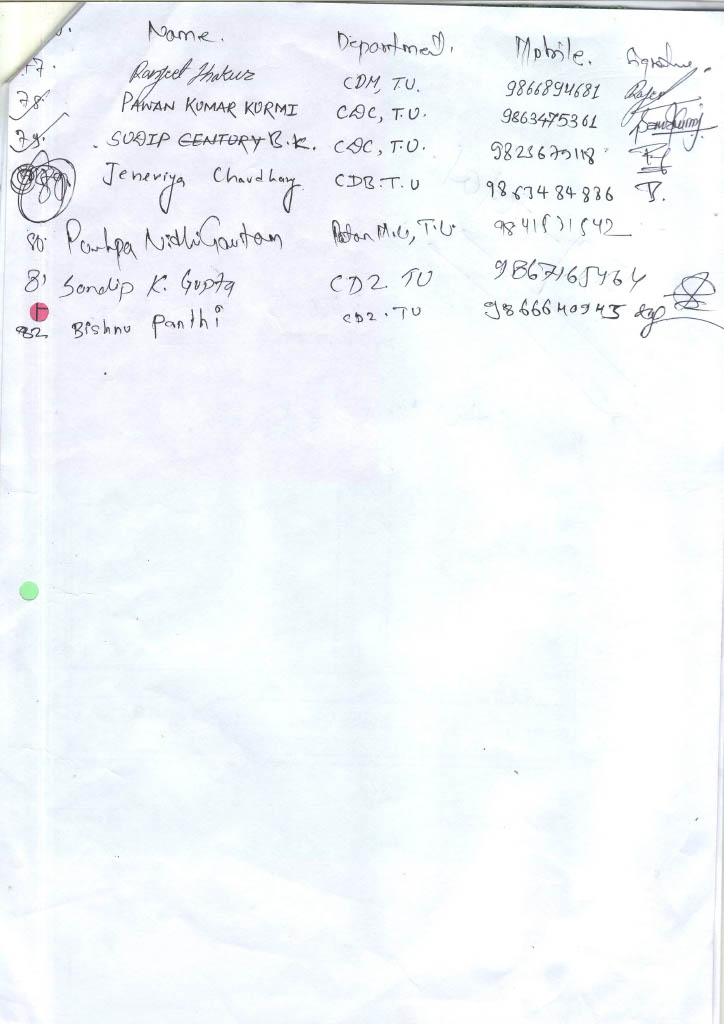
\includegraphics[width=12cm, height=12cm]{4.jpg}
\end{figure}



\end{document}



%%% Local Variables:
%%% mode: latex
%%% TeX-master: t
%%% End:
